\documentclass[11pt,fontset=fandol]{ctexart}
\usepackage[a4paper,margin=1in]{geometry}
\usepackage{amsmath,amssymb,amsfonts}
\usepackage{booktabs}
\usepackage{graphicx}
\usepackage{caption}
\usepackage{enumitem}
\usepackage[table]{xcolor}
\usepackage{array}
\usepackage[hidelinks]{hyperref}
\usepackage{xurl}
\usepackage{microtype}

\title{二维 One-/Two-Target Gating 机制整合报告\\\large one-target 回退到共享对称基线与非极端非对称对照}
\author{}
\date{}

\setlist{nosep}
\setlength{\textfloatsep}{8pt plus 2pt minus 2pt}
\setlength{\floatsep}{6pt plus 2pt minus 2pt}
\setlength{\intextsep}{6pt plus 2pt minus 2pt}
\setlength{\abovecaptionskip}{4pt}
\setlength{\belowcaptionskip}{0pt}
\setlength{\tabcolsep}{5pt}
\renewcommand{\arraystretch}{1.10}

\begin{document}
\maketitle

\section*{结论先行}
这一稿继续保留 March 16 的来源链
\texttt{二维半透膜\_gating\_game}
$\rightarrow$
\texttt{two\_target\_gating\_framework}
$\rightarrow$
\texttt{one\_two\_target\_deepening\_work}，
但 one-target 主文已经回退到一个更稳的配置体系：
\begin{itemize}
  \item \textbf{标准配置} 固定为共享对称基线 \texttt{sym\_shared}，而不是极端非对称点；
  \item \textbf{两类非对称} 分开讲：一类是 top/bottom 不对称，另一类是同一条膜上的 direction 不对称；
  \item \textbf{第一峰} 现在可以更明确地解释成 corridor fast branch；
  \item \textbf{第二峰} 的主体不是“纯穿膜峰”，而是左端开口 detour/rollback 支路，半透膜 crossing 主要是次级修饰；
  \item \textbf{rollback} 恢复为 one-target 的主要离散机制语言，而且是 \emph{gate-free} 的：离开起始盆地 $A$ 后是否又返回 $A$；
  \item \textbf{x-gate} 仍然保留，但只承担时间锚点机制：解释第一次 leak 发生在过门前还是过门后；
  \item \textbf{双峰丢失} 统一按 \texttt{phase=0} 定义；\texttt{phase=1} 只表示弱化，不表示 second peak 已经消失。
\end{itemize}

\section{来源链与当前定位}
\paragraph{为什么这一稿要重新改写 one-target。}
前一轮 canonical 化已经把 6 个下载文件吸收到仓库共享代码与标准 report 目录里，但 one-target 的主叙事仍然不够稳：一方面，极端的 $\kappa=0$ 点过于“展示化”；另一方面，把 rollback 绑在 $x=X_g$ gate 上容易造成概念混乱。这一稿的目标就是把 one-target 拉回到更物理、更接近仓库既有风格的语言。

\begin{figure}[!htbp]
  \centering
  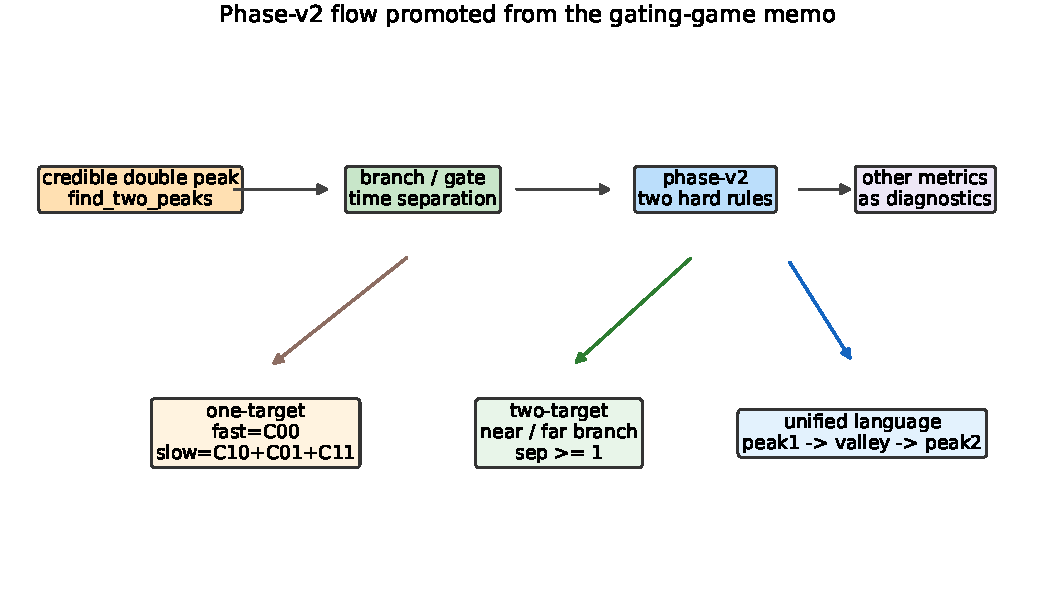
\includegraphics[width=0.84\linewidth]{../artifacts/figures/gating_game_phase_v2_flow.pdf}
  \caption{来源链中的 phase-v2 / gating-game 结构图。当前 canonical 稿保留这条来源链，但不再让 one-target 主机制完全受旧的 gate 语言牵引。}
\end{figure}

\begin{figure}[!htbp]
  \centering
  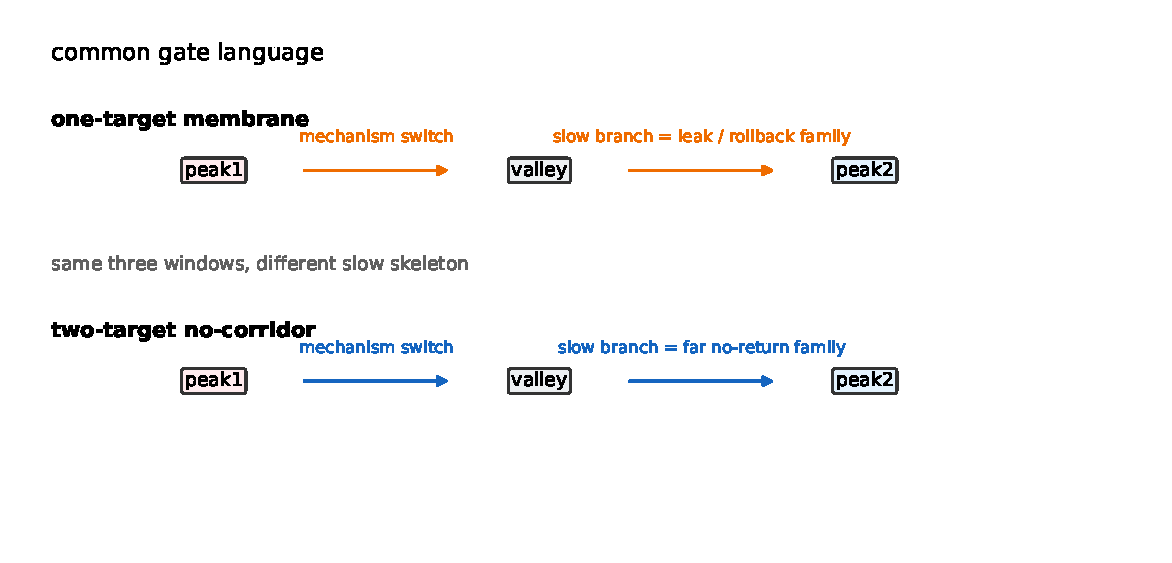
\includegraphics[width=0.92\linewidth]{../artifacts/figures/unified_mechanism_ladder.pdf}
  \caption{统一机制阶梯。two-target 仍沿用 gate-lifted family 语言；one-target 则回退到“共享对称基线 + rollback 主分类 + x-gate 辅线”这套更稳定的仓库口径。}
\end{figure}

\section{one-target 的标准配置与两种对称性}
\paragraph{标准配置是什么。}
当前 one-target 的唯一标准配置是
\[
\texttt{sym\_shared}:\qquad
\kappa_{\rm top}=\kappa_{\rm bottom}=k_{\rm ref}=0.002,
\]
并且在 directional 口径下同样满足
\[
\kappa_{c\to o}=\kappa_{o\to c}=0.002.
\]
也就是说，\texttt{sym\_shared} 同时是 top/bottom 对称和 same-membrane directional 对称的共享基线。

\paragraph{为什么不再把 $\kappa=0$ 当 canonical 代表点。}
极端点当然仍然有研究价值，但它们更适合做 control 或 loss boundary，不适合做主代表点。当前 canonical 代表点全部来自固定扫描规则：
\begin{itemize}
  \item 优先选 \texttt{phase=2}；
  \item 优先选参数都大于 $0$ 的内点，而不是贴着边界；
  \item 优先选与固定 balanced anchor 最近、但同时 separation 仍然足够清楚的点；
  \item 如果 anchor 本身不在 \texttt{phase=2}，就选同方向、同网格上最近的 \texttt{phase=2} 内点。
\end{itemize}
所以当前的非对称代表点不再是“把一边直接关死”的极端图，而是 non-extreme comparison cases。

\begin{table}[!htbp]
  \centering
  \caption{one-target canonical representative cases。这里明确区分标准配置与比较配置，并给出每个代表点的实际参数、phase 与 separation。}
  \begin{tabular}{lllrrllr}
\toprule
case & role & parameters & phase & sep & peak2 rollback & peak2 gate & rollback \\
\midrule
shared symmetric baseline & standard & $(\kappa_{c\to o},\kappa_{o\to c})=(0.0020,0.0020)$ & 2 & 1.528 & L0R1 & N & 89.2\% \\
top/bottom balanced asymmetry & comparison & $(\kappa_{top},\kappa_{bottom})=(0.0020,0.0005)$ & 2 & 1.689 & L0R1 & N & 89.1\% \\
directional easy-out / hard-return & comparison & $(\kappa_{c\to o},\kappa_{o\to c})=(0.0020,0.0005)$ & 2 & 1.614 & L0R1 & N & 89.3\% \\
directional hard-out / easy-return & comparison & $(\kappa_{c\to o},\kappa_{o\to c})=(0.0005,0.0020)$ & 2 & 1.737 & L0R1 & N & 88.9\% \\
\bottomrule
\end{tabular}

\end{table}

\begin{figure}[!htbp]
  \centering
  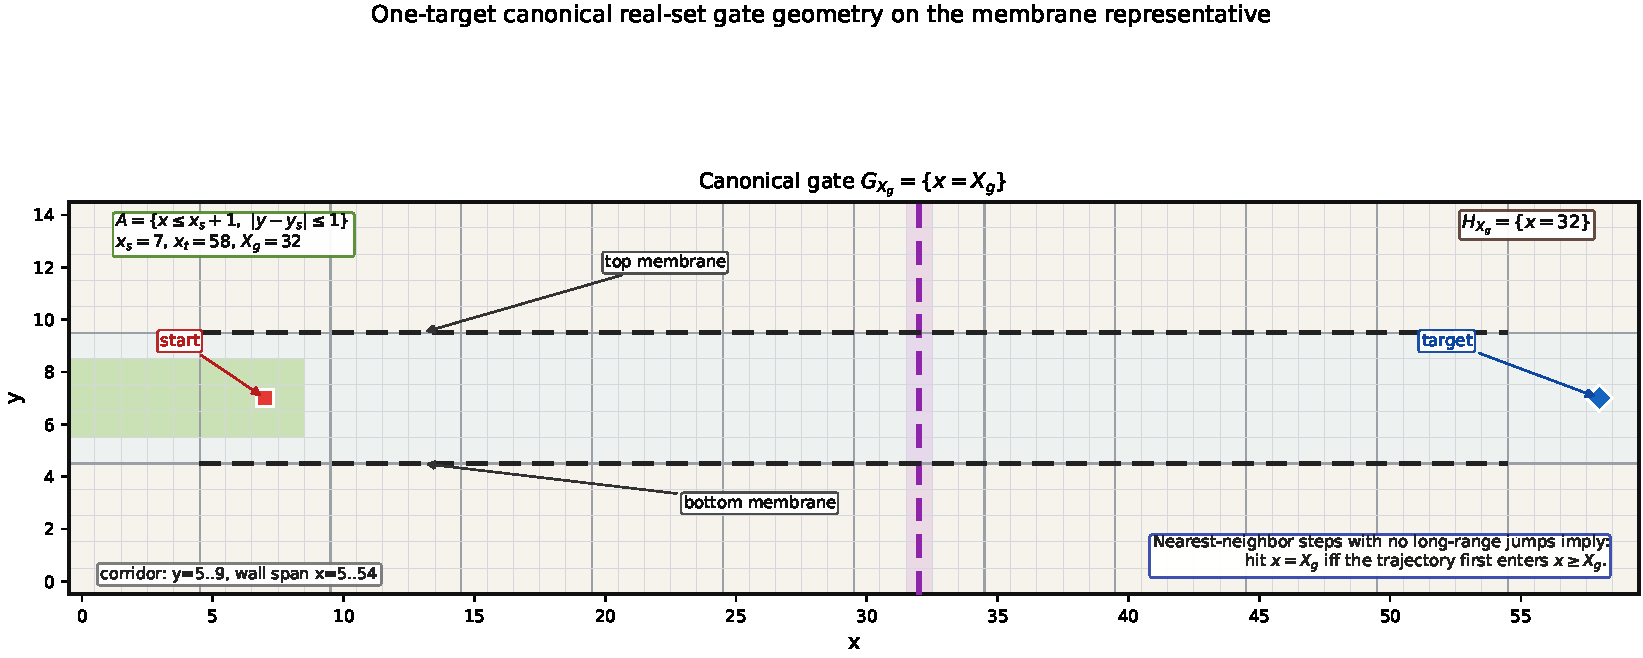
\includegraphics[width=0.90\linewidth]{../artifacts/figures/one_target_gate_geometry.pdf}
  \caption{one-target 的标准配置图。主图使用共享对称基线 \texttt{sym\_shared}，并明确标出格点、corridor、起始盆地 $A$、target、上下真实半透膜，以及 canonical x-gate $G_{X_g}=\{x=X_g\}$。}
\end{figure}

\paragraph{这两种“对称/非对称”具体指什么。}
这一稿 one-target 把两条不同的对称性彻底分开：
\begin{enumerate}
  \item \textbf{top/bottom symmetry}：上膜和下膜是否相同；
  \item \textbf{same-membrane directional symmetry}：同一条膜上，\texttt{corridor$\to$outside} 与 \texttt{outside$\to$corridor} 是否相同。
\end{enumerate}
前者对应 \texttt{tb} 参数平面 $(\kappa_{\rm top},\kappa_{\rm bottom})$，后者对应 \texttt{dir} 参数平面 $(\kappa_{c\to o},\kappa_{o\to c})$。这两个平面数值上不一样，也对应不同的物理问题。

\section{gate-free rollback 4 类与 x-gate 3 类}
\paragraph{为什么 rollback 现在不再依赖 gate。}
这一稿把 rollback 改成真正 gate-free 的定义：轨迹离开起始盆地 $A$ 之后，后来是否又重新进入 $A$。这样定义以后，rollback 不再需要先“命中某个 gate”，因此 4 类
\[
L0R0,\quad L0R1,\quad L1R0,\quad L1R1
\]
是互斥且完备的：
\begin{itemize}
  \item $L0R0$：无 leak，且无 return-to-$A$；
  \item $L0R1$：无 leak，但离开 $A$ 后又回到 $A$；
  \item $L1R0$：有 leak，但之后没有回到 $A$；
  \item $L1R1$：有 leak，且之后回到 $A$。
\end{itemize}

\paragraph{x-gate 现在负责什么。}
x-gate 仍然保留，但它只做一件事：把 leak 的第一次发生时间相对于
\[
G_{X_g}=\{x=X_g\}
\]
这条真实截线来记账。于是得到
\[
N=\text{NoLeak},\qquad
P=\text{first leak before gate},\qquad
Q=\text{first leak after gate}.
\]
在当前最近邻格点动力学下，命中 $x=X_g$ 与首次进入 $x\ge X_g$ 是等价事件，所以主文只保留一条 canonical x-gate 机制线。

\begin{figure}[!htbp]
  \centering
  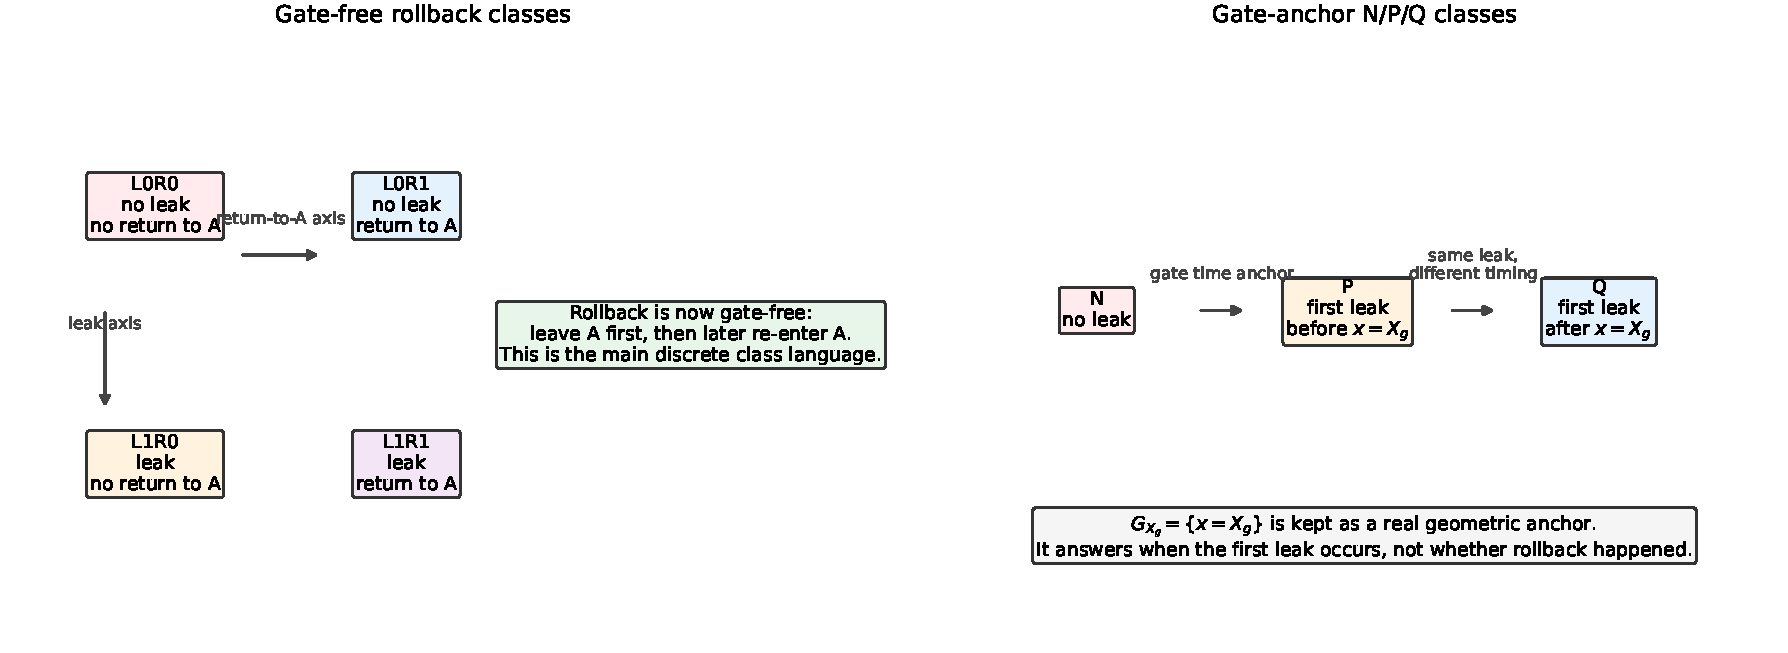
\includegraphics[width=0.88\linewidth]{../artifacts/figures/one_target_class_crosswalk.pdf}
  \caption{one-target class explainer。rollback 4 类回答“有没有 leak、有没有返回 $A$”；$N/P/Q$ 回答“第一次 leak 相对 x-gate 发生在什么时候”。两者并列，但不再互相定义。}
\end{figure}

\section{top/bottom 参数扫描}
\paragraph{这组扫描回答什么。}
这组 $15\times 15$ 参数平面扫描固定在
\[
\kappa_{\rm top},\kappa_{\rm bottom}\in
\{0,0.00025,\ldots,0.005\},
\]
回答的是：上下两条膜的通透性如何改变 one-target 的 double-peak 强度、phase0 失效区和 rollback/gate 机制。

\begin{figure}[!htbp]
  \centering
  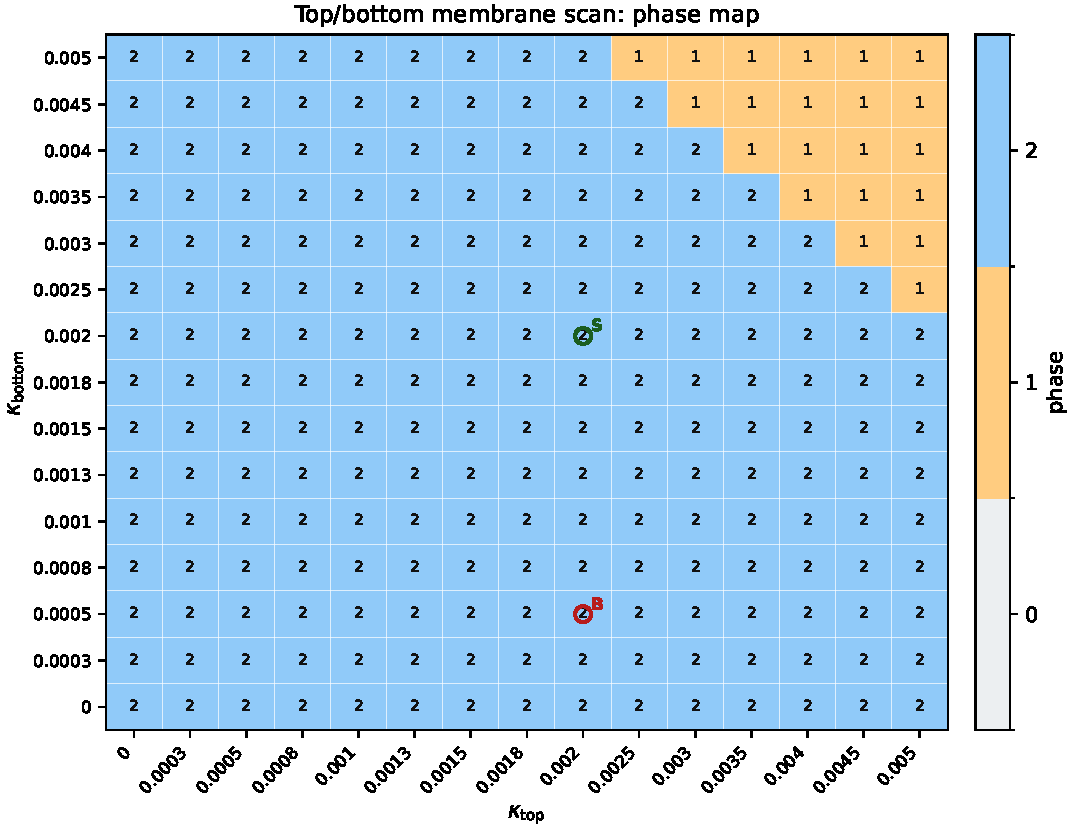
\includegraphics[width=0.88\linewidth]{../artifacts/figures/one_target_tb_phase_map.pdf}
  \caption{top/bottom 参数平面的 phase map。标准配置 \texttt{sym\_shared} 和 balanced top-open 对照点都在图中明确标出。}
\end{figure}

\begin{figure}[!htbp]
  \centering
  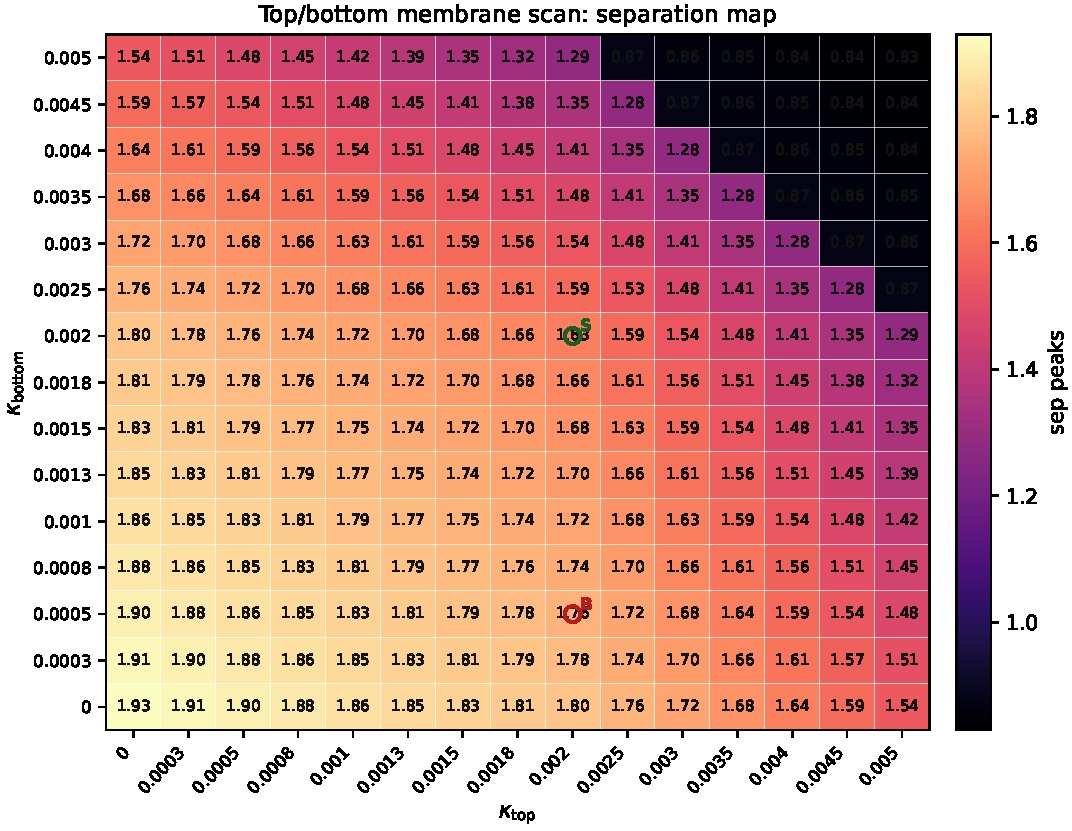
\includegraphics[width=0.88\linewidth]{../artifacts/figures/one_target_tb_sep_map.pdf}
  \caption{同一参数平面的 peak separation map。这里的颜色变化告诉我们：从 shared symmetric baseline 往非对称方向走时，double-peak 是先弱化，再在某些区域真正掉进 \texttt{phase=0}。}
\end{figure}

\section{same-membrane directional 参数扫描}
\paragraph{这组扫描为什么单独保留。}
如果只看 top/bottom，不足以回答“同一条膜是易出难回还是难出易回”这类更精细的问题。因此我们单独扫
\[
\kappa_{c\to o},\kappa_{o\to c}\in
\{0,0.00025,\ldots,0.005\}.
\]
这条扫描直接回答 same-membrane directional asymmetry 如何改变 slow branch。

\begin{figure}[!htbp]
  \centering
  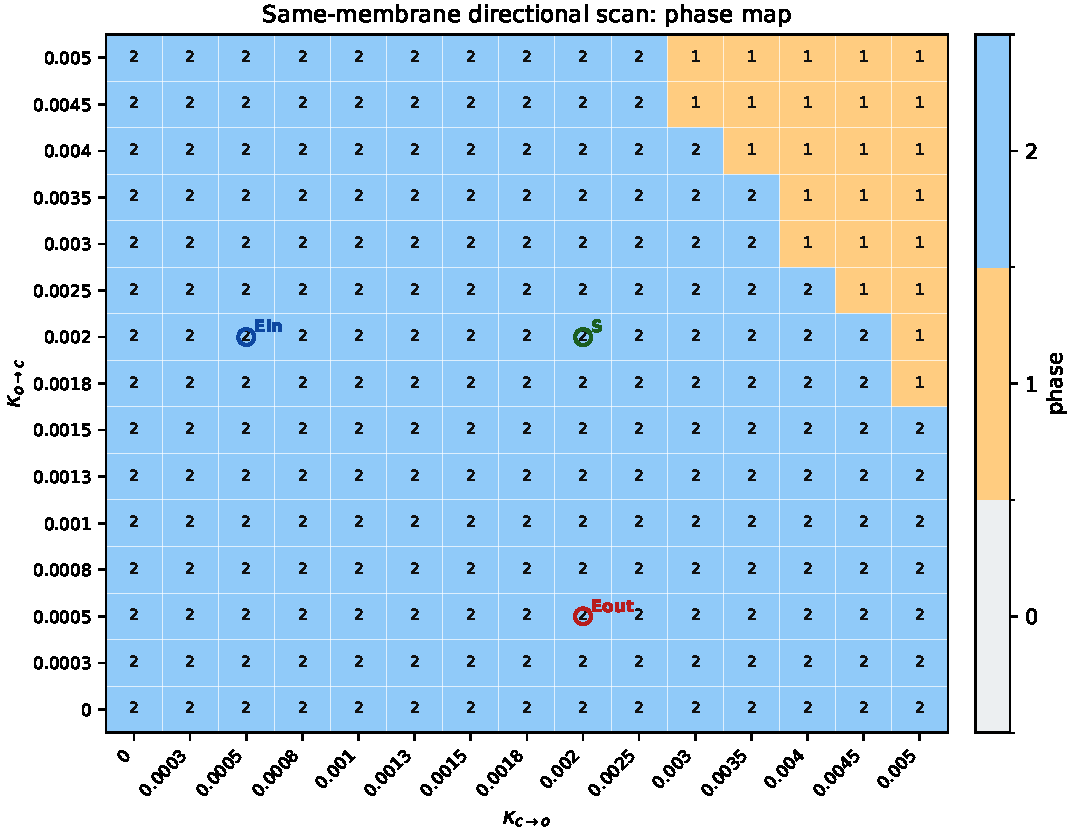
\includegraphics[width=0.88\linewidth]{../artifacts/figures/one_target_dir_phase_map.pdf}
  \caption{same-membrane directional 参数平面的 phase map。共享对称基线和 two directional comparison cases 均已标出。}
\end{figure}

\begin{figure}[!htbp]
  \centering
  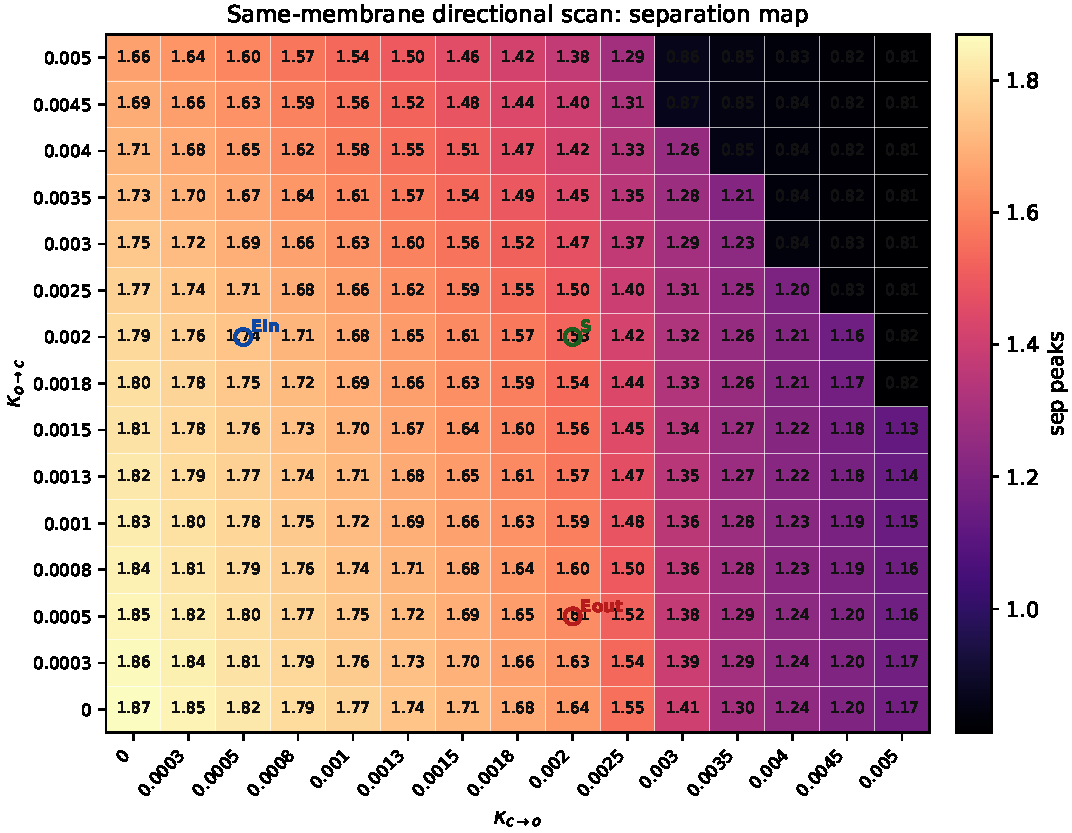
\includegraphics[width=0.88\linewidth]{../artifacts/figures/one_target_dir_sep_map.pdf}
  \caption{directional 参数平面的 peak separation map。它直接显示 easy-out / easy-in 如何改变双峰清晰度。}
\end{figure}

\begin{table}[!htbp]
  \centering
  \caption{x-gate 全扫描的 summary。对每个 canonical case，表中汇报 dominant $N$ 计数以及 $P/Q/rollback$ 的变化范围。}
  \begin{tabular}{llrrrr}
\toprule
case & scan range & dom. $N$ & $P$ range & $Q$ range & rollback range \\
\midrule
directional hard-out / easy-return & 9..57 & 49 & 0.1\%--2.8\% & 2.5\%--5.2\% & 28.2\%--76.4\% \\
directional easy-out / hard-return & 9..57 & 49 & 0.1\%--8.0\% & 1.3\%--9.1\% & 27.8\%--77.2\% \\
shared symmetric baseline & 9..57 & 49 & 0.2\%--8.6\% & 2.9\%--11.4\% & 27.5\%--77.0\% \\
top/bottom balanced asymmetry & 9..57 & 49 & 0.1\%--5.4\% & 1.8\%--7.2\% & 28.0\%--76.8\% \\
\bottomrule
\end{tabular}

\end{table}

\begin{figure}[!htbp]
  \centering
  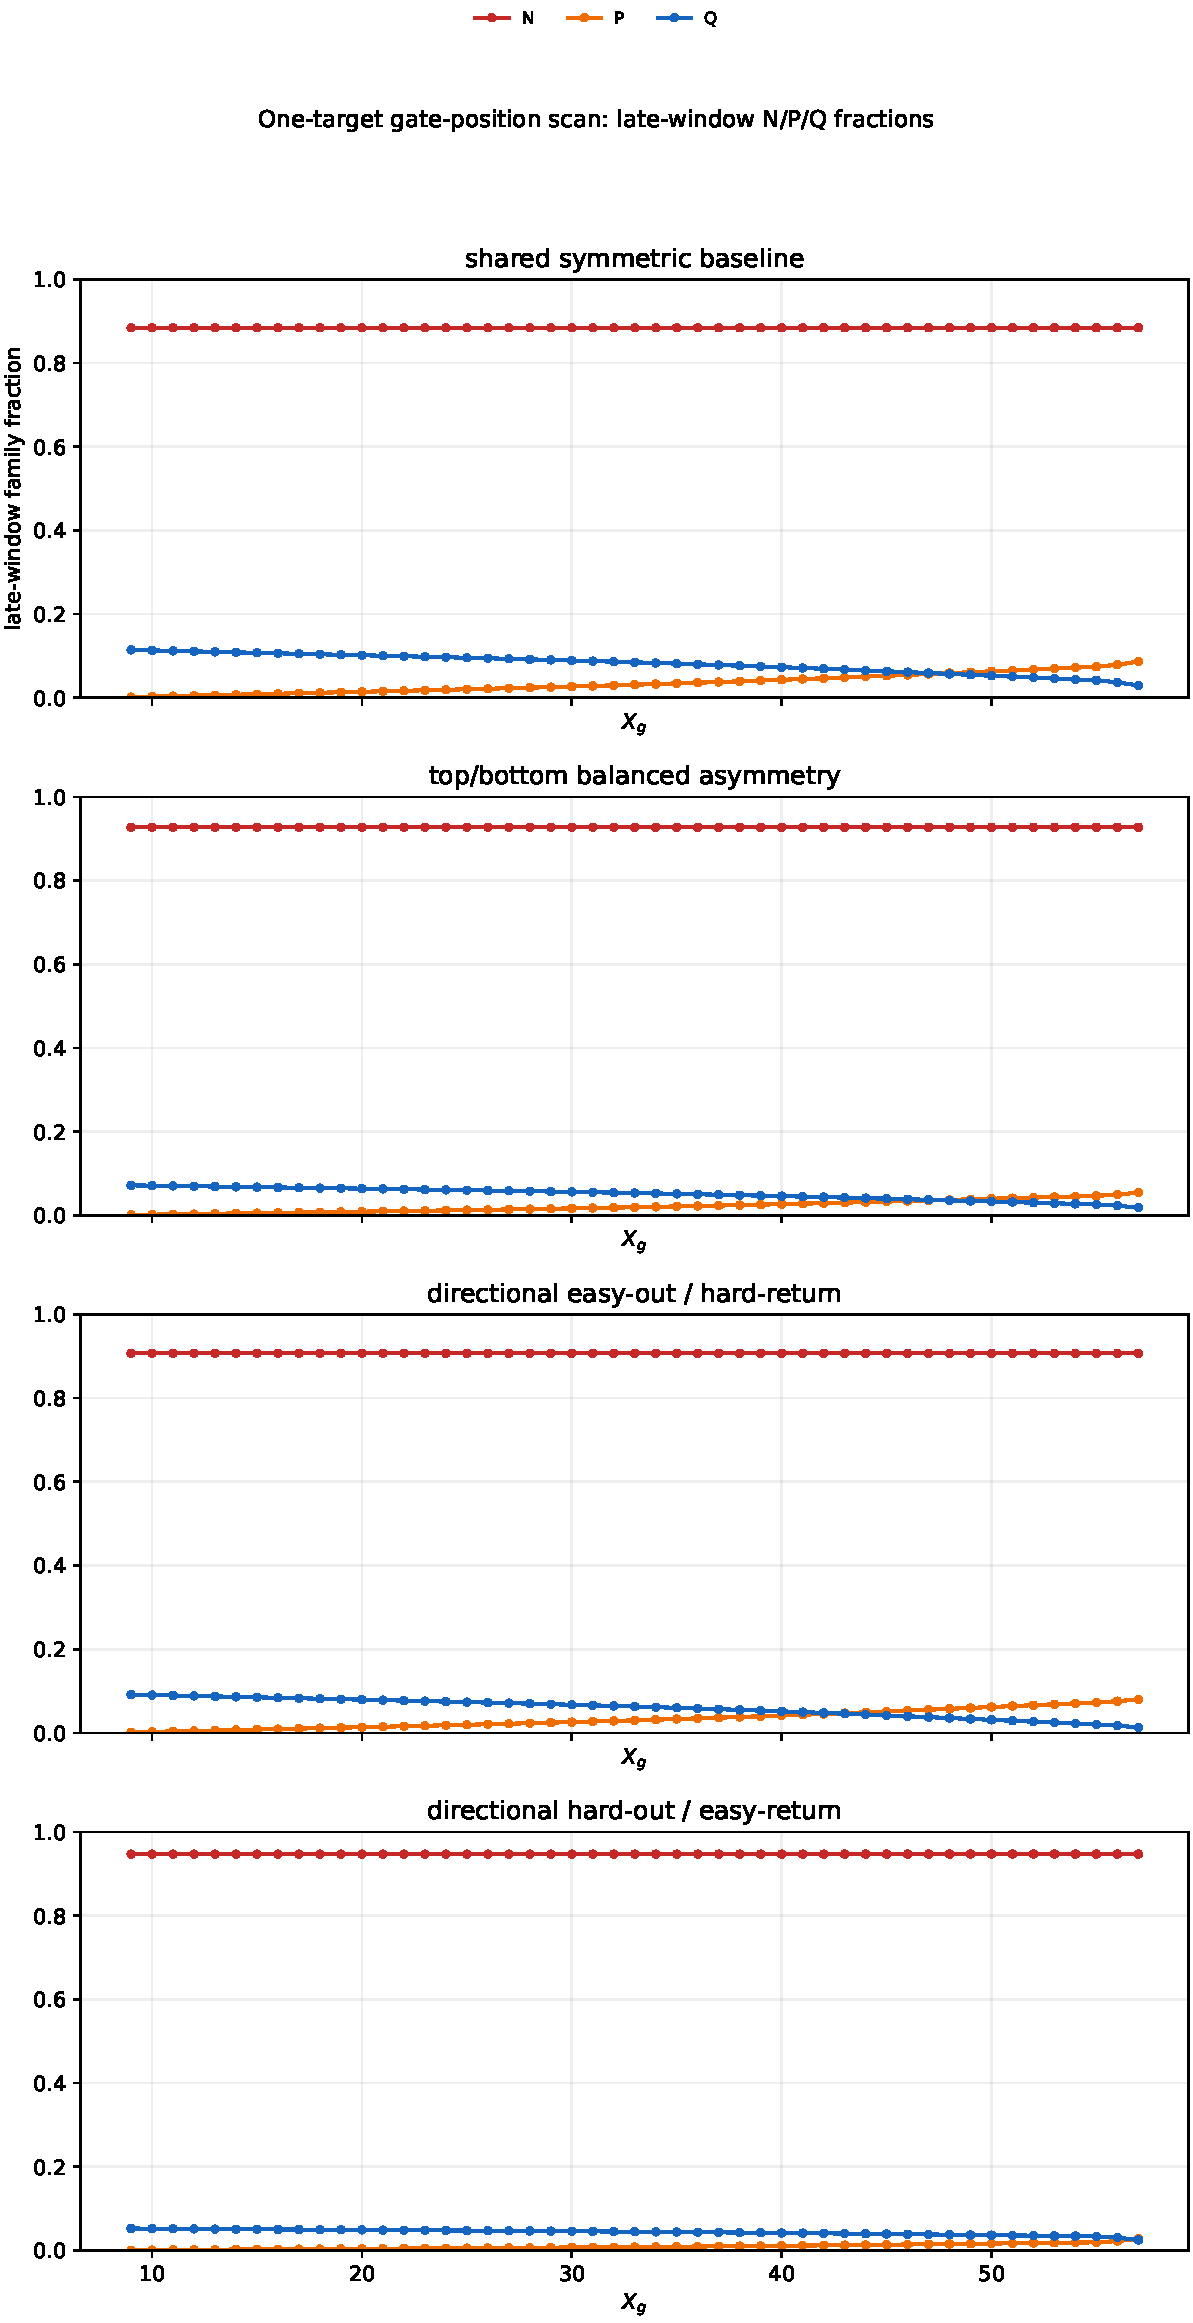
\includegraphics[width=0.92\linewidth]{../artifacts/figures/one_target_gate_scan_families.pdf}
  \caption{$X_g$ 全扫描下的 $N/P/Q$ 分解。当前 canonical 结果清楚表明：x-gate 更像一个几何时间锚点，而不是强分相器；它主要重分配 $P/Q$ 质量。}
\end{figure}

\begin{figure}[!htbp]
  \centering
  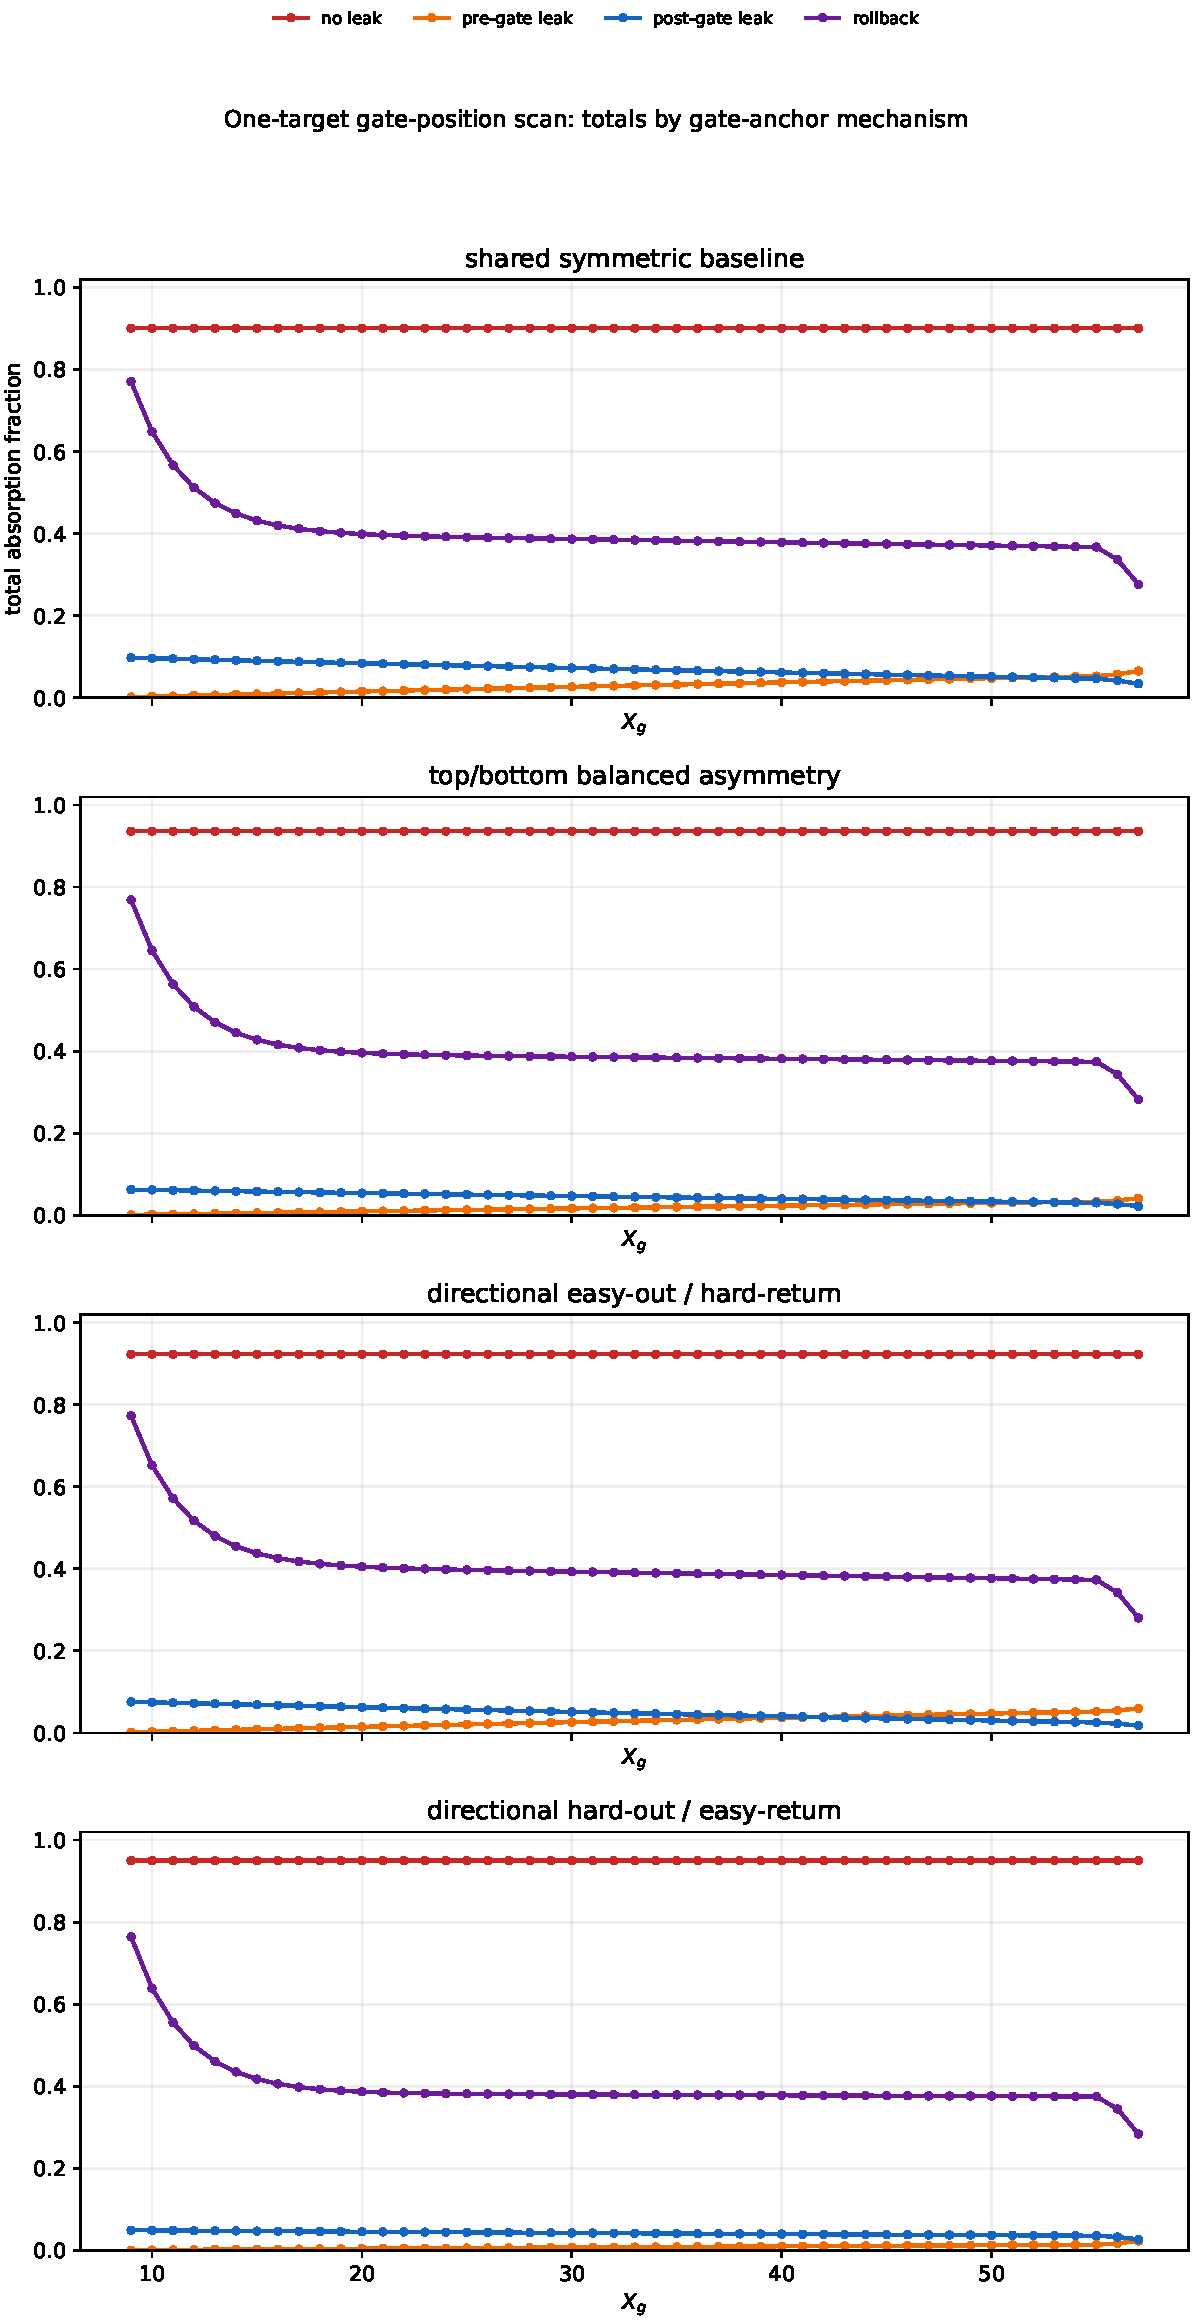
\includegraphics[width=0.92\linewidth]{../artifacts/figures/one_target_gate_scan_totals.pdf}
  \caption{同一组 $X_g$ 扫描下的总量图。这里直接回答“调整 gate 位置以后比例有没有变化”：有，但主要体现在 $P/Q$ 预算与 rollback 总量上，而不是 dominant family 翻转。}
\end{figure}

\section{起点扫描与 phase0：双峰何时真正丢失}
\paragraph{这一节只把 \texttt{phase=0} 当成双峰丢失。}
当前稿里，\texttt{phase=2} 表示 clear double peak，\texttt{phase=1} 表示弱化但 second peak 仍在；只有 \texttt{phase=0} 才表示双峰真正丢失。因此，“什么时候丢失双峰”的问题在本稿里被严格解释成：哪些参数区和哪些起点位置先掉进 \texttt{phase=0}。

\begin{figure}[!htbp]
  \centering
  
\includegraphics[width=0.95\linewidth]{../artifacts/figures/one_target_start_phase_map.pdf}
  \caption{四个 canonical cases 的完整起点 phase atlas。它直接回答：在不同膜配置下，phase0 是先从哪里出现、再如何扩展。}
\end{figure}

\paragraph{为什么这里不再画整张 leak-balance atlas。}
起点扫描这一节的主要任务是回答 ``phase0 从哪里先出现''。因此这一轮 canonical 重构把 full start atlas 保持为 phase-only exact；更细的 leak timing 与 rollback 预算，统一放到参数扫描与代表窗口分解里解释，而不再对每一个起点格点都重复做一次重型 exact 机制 lift。

\begin{table}[!htbp]
  \centering
  \caption{phase0 loss summary。每个 canonical case 都给出 centerline onset、off-axis loss 与 target-adjacent collapse 的代表位置。}
  \begin{tabular}{lllll}
\toprule
case & phase-0 onset & off-axis loss & target-adjacent collapse & phase counts \\
\midrule
shared symmetric baseline & (46, 7) & (47, 5) & (57, 7) & 0:81/1:558/2:320 \\
top/bottom balanced asymmetry & (46, 7) & (46, 5) & (57, 7) & 0:83/1:555/2:321 \\
directional easy-out / hard-return & (46, 7) & (47, 5) & (57, 7) & 0:80/1:562/2:317 \\
directional hard-out / easy-return & (47, 7) & (47, 5) & (57, 7) & 0:77/1:555/2:327 \\
\bottomrule
\end{tabular}

\end{table}

\section{代表点细化：rollback、x-gate 与 directional flux}
\paragraph{哪条机制更强。}
当前 canonical 结果下，one-target 更强的离散主机制是 gate-free rollback 4 类，而不是 x-gate 本身。原因很简单：rollback 4 类直接回答“有没有 leak、有没有返回 $A$”，辨识力更稳定；x-gate 更像时间锚点，主要解释 leak 发生在 gate 前还是 gate 后。

\begin{figure}[!htbp]
  \centering
  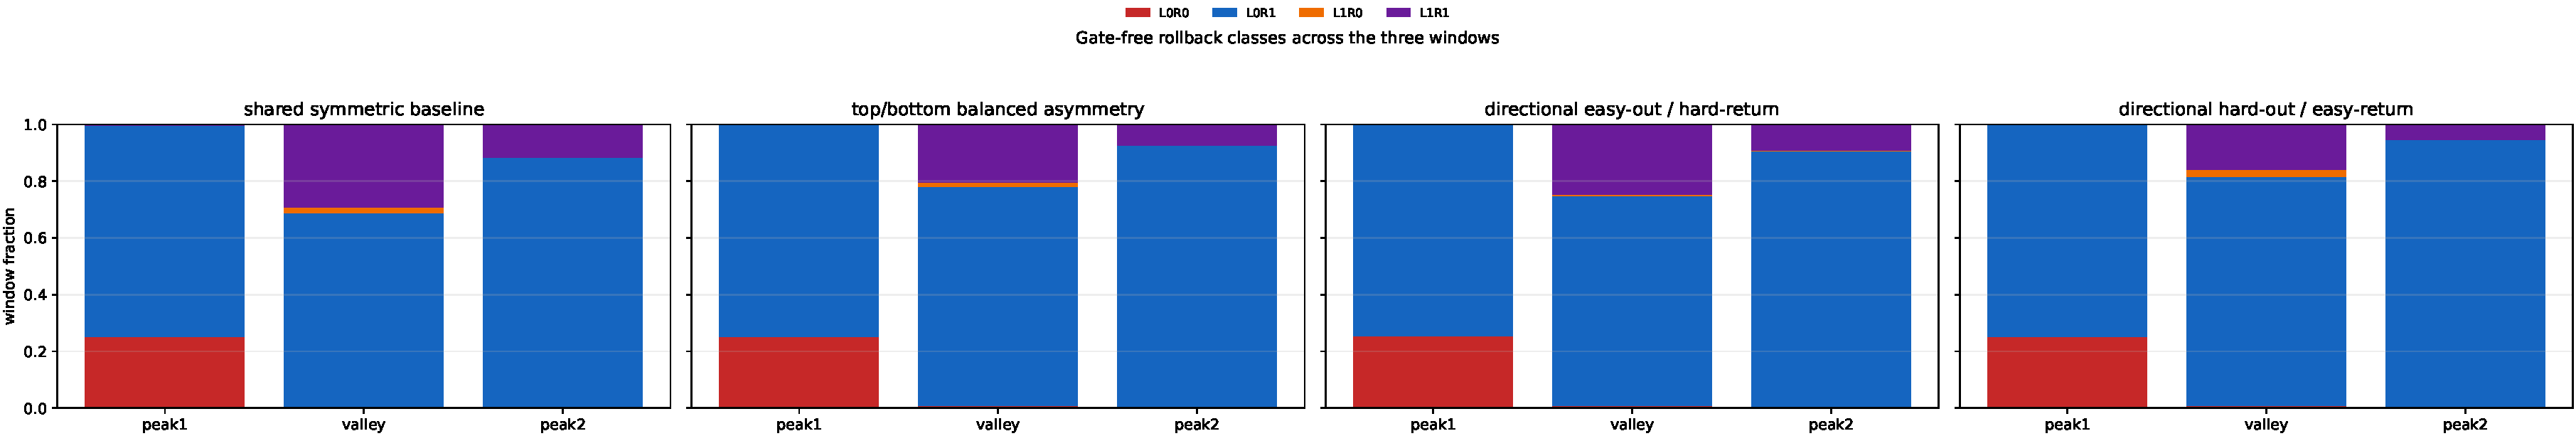
\includegraphics[width=0.92\linewidth]{../artifacts/figures/one_target_rollback_window_bars.pdf}
  \caption{代表点的 rollback 4 类三窗口分解。这里的 $L0R1+L1R1$ 直接衡量“离开 $A$ 之后又回到 $A$”在 valley / peak2 的占比。}
\end{figure}

\begin{figure}[!htbp]
  \centering
  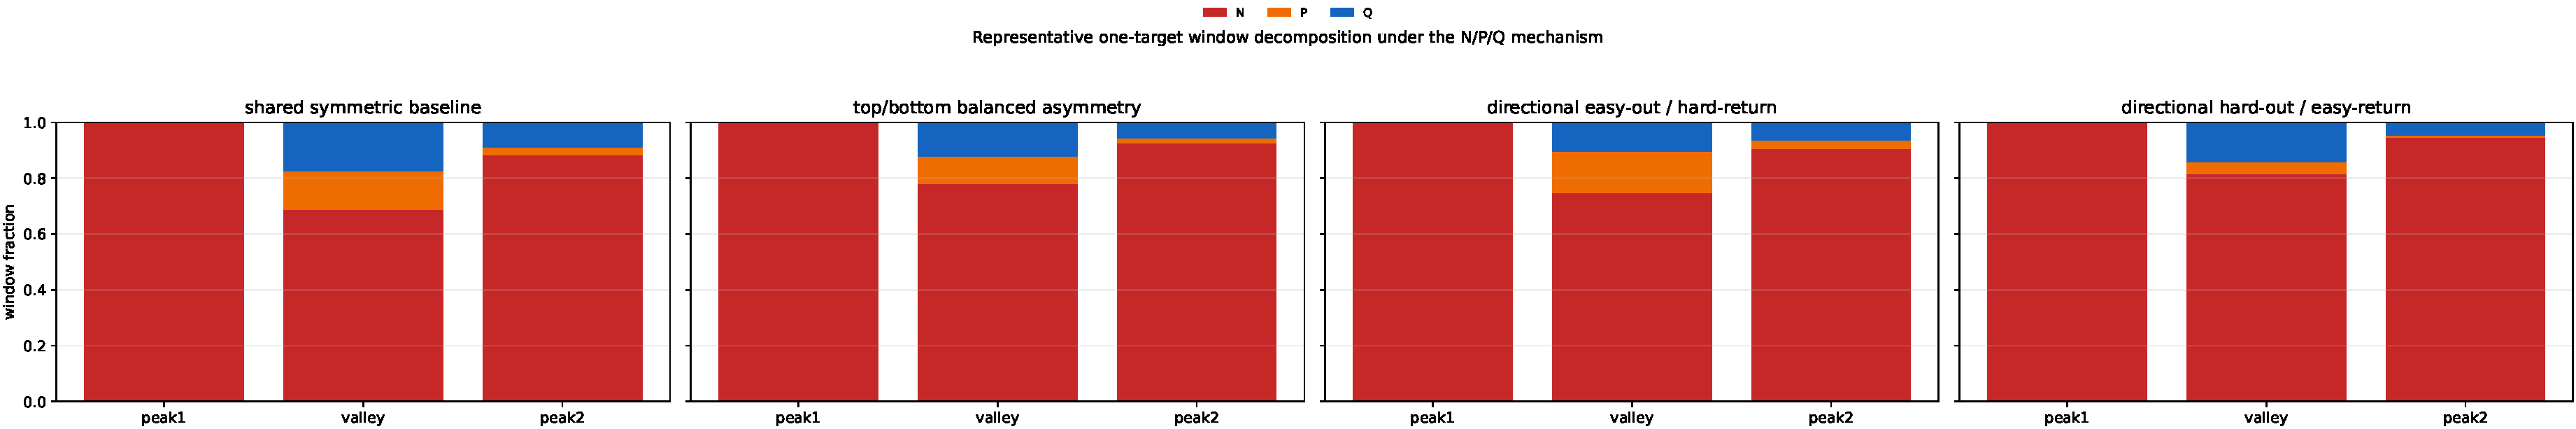
\includegraphics[width=0.92\linewidth]{../artifacts/figures/one_target_window_families.pdf}
  \caption{代表点的 x-gate 三窗口分解。$N/P/Q$ 不是主离散分类，而是解释第一次 leak 相对 gate 发生时序的辅线。}
\end{figure}

\begin{figure}[!htbp]
  \centering
  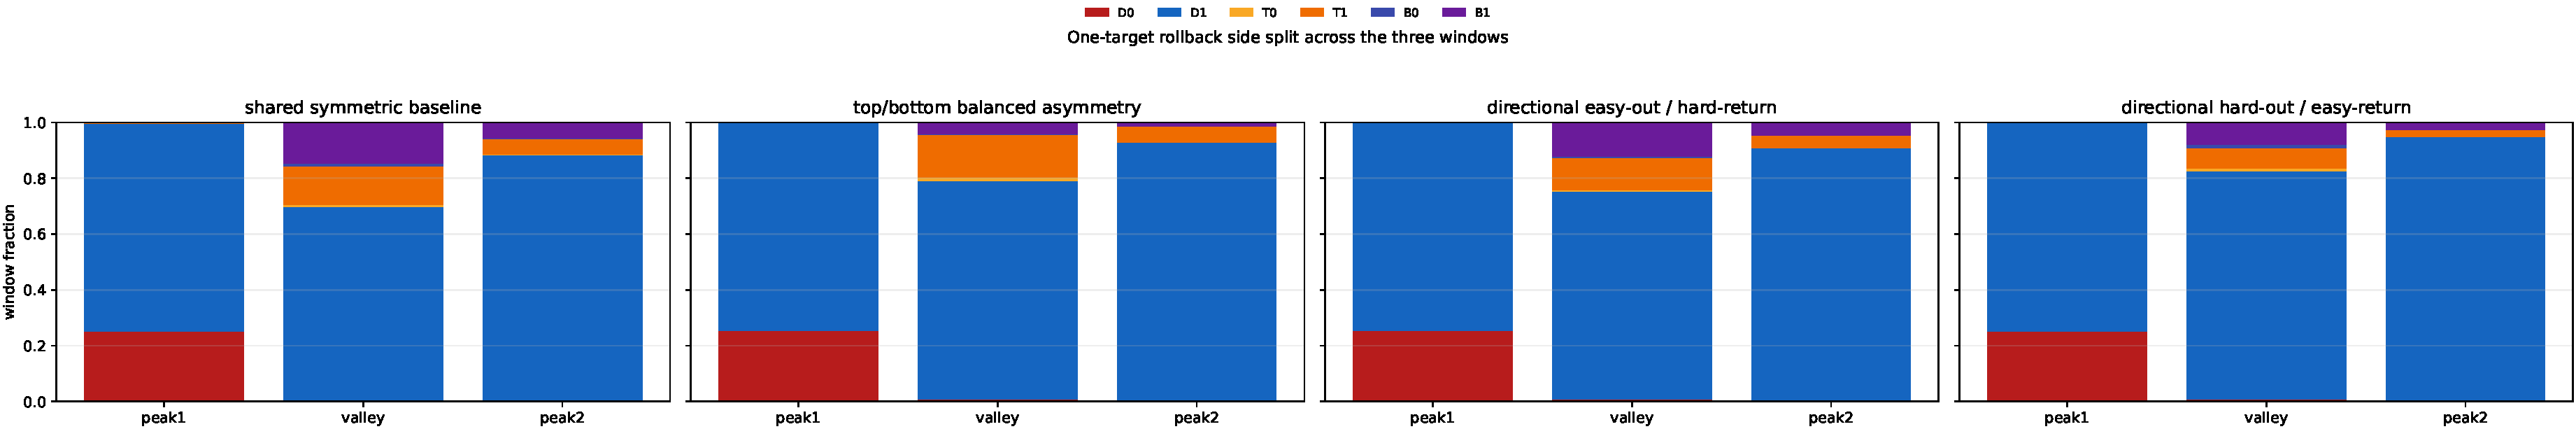
\includegraphics[width=0.92\linewidth]{../artifacts/figures/one_target_side_window_bars.pdf}
  \caption{rollback side-aware 细化。对 shared symmetric baseline 来说，top/bottom 主要是对称性检查；对 top/bottom 非对称 case 来说，它才真正体现 side preference。}
\end{figure}

\begin{figure}[!htbp]
  \centering
  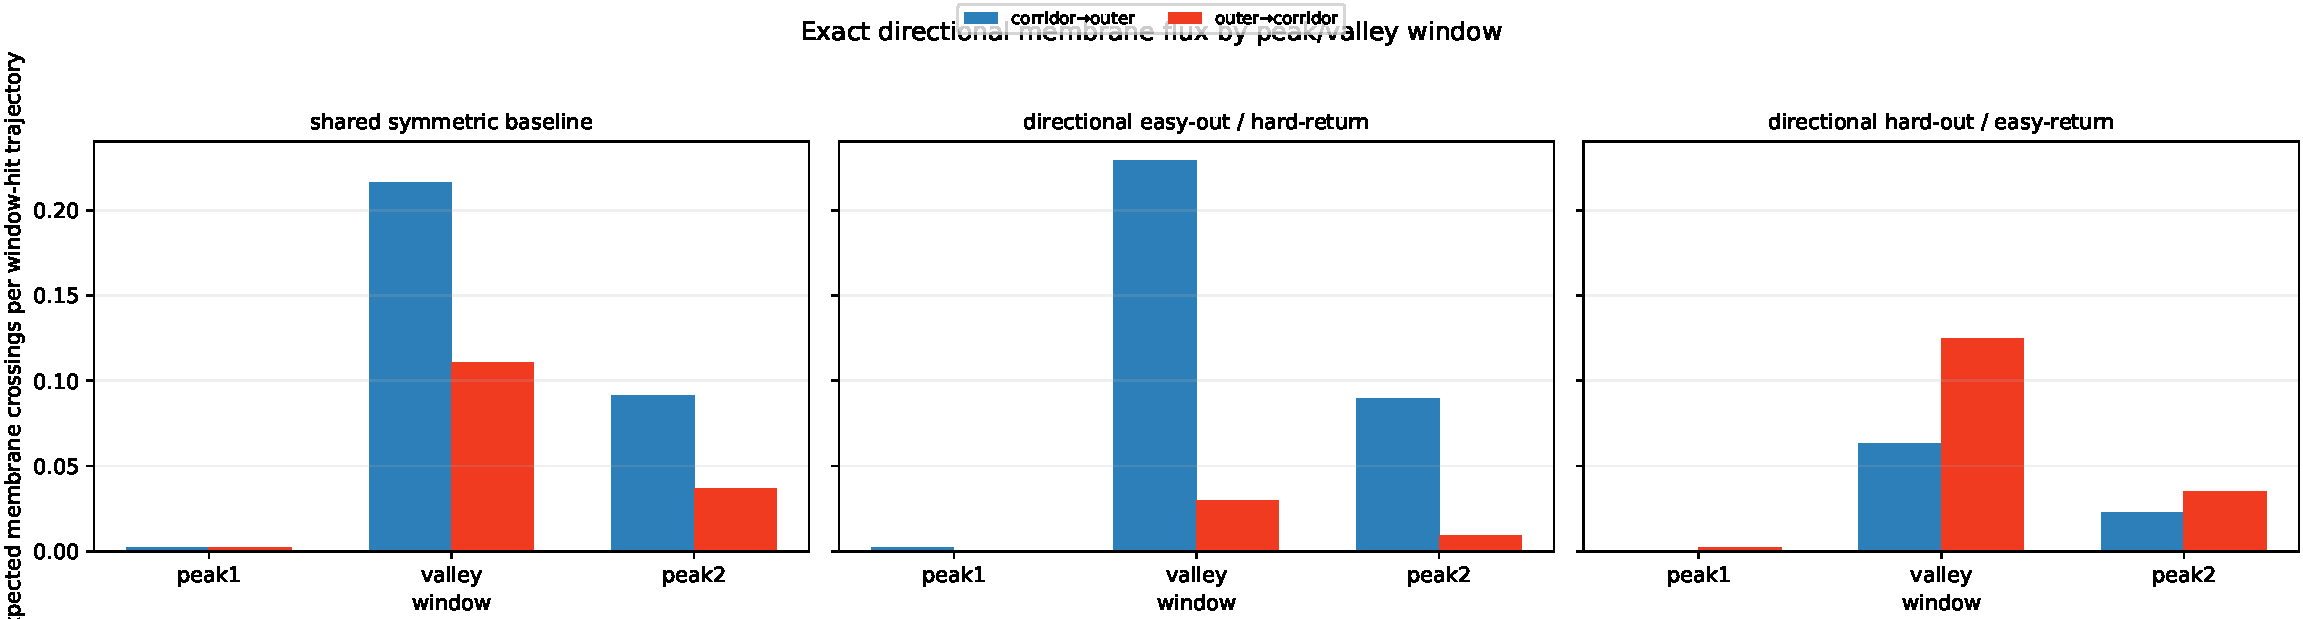
\includegraphics[width=0.92\linewidth]{../artifacts/figures/one_target_directional_window_flux.pdf}
  \caption{directional window flux diagnostics。它直接解释 easy-out / easy-in 为什么会改变 second peak，而不只停留在参数名层面。}
\end{figure}

\begin{figure}[!htbp]
  \centering
  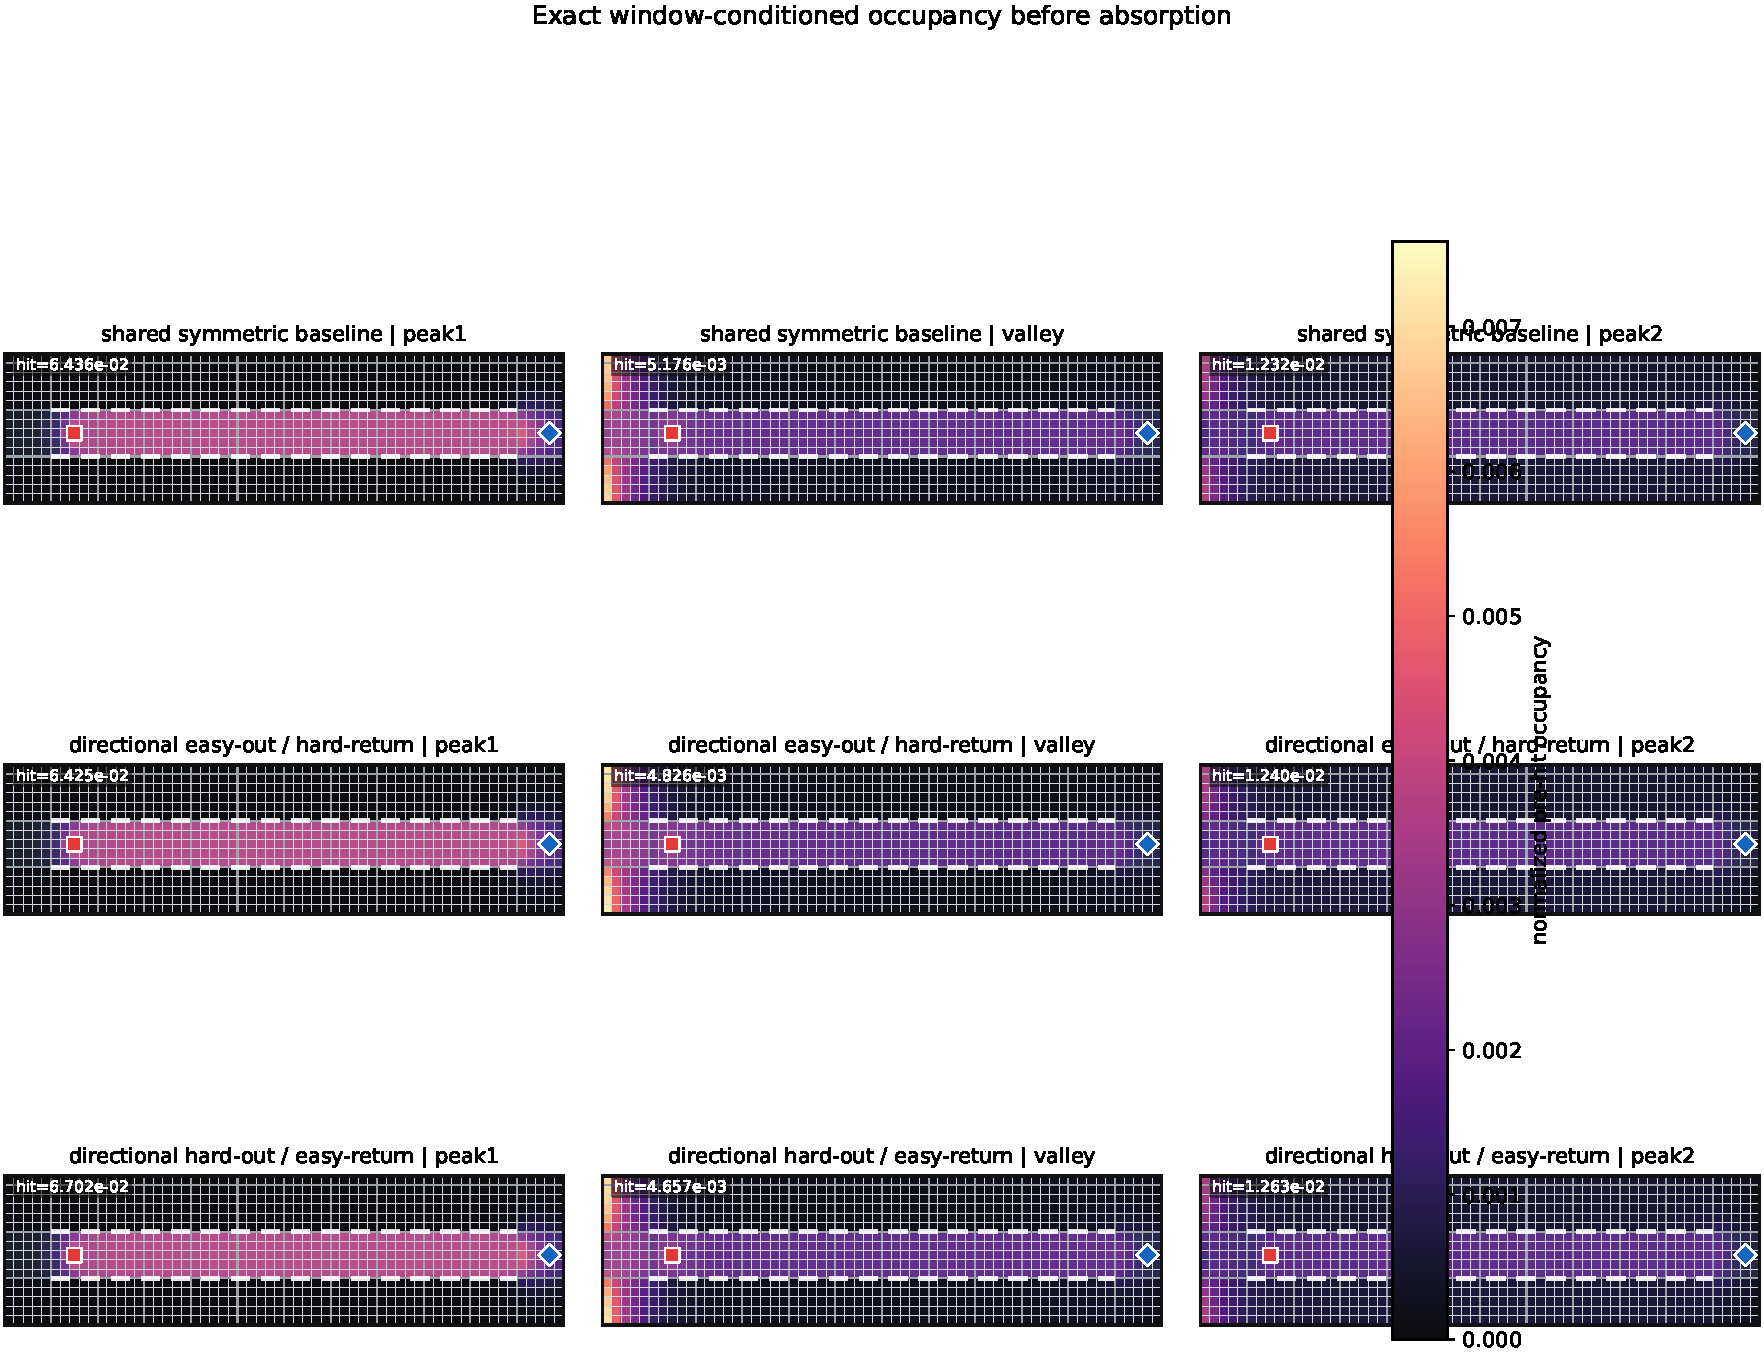
\includegraphics[width=0.95\linewidth]{../artifacts/figures/one_target_directional_window_occupancy_atlas.pdf}
  \caption{代表 case 的窗口 occupancy atlas。它把 directional slow branch 的空间位置重新画回真实格点几何。}
\end{figure}

\begin{table}[!htbp]
  \centering
  \caption{one-target representative recheck。这里汇报 phase、separation、peak2 rollback share，以及 $X_g$ 扫描下的 $P/Q/rollback$ 变化范围。}
  \begin{tabular}{lrrrrrr}
\toprule
case & phase & sep & peak2 rollback share & $P$ range & $Q$ range & rollback range \\
\midrule
shared symmetric baseline & 2 & 1.633 & 99.7\% & 0.2\%--8.7\% & 3.1\%--11.6\% & 27.7\%--77.1\% \\
top/bottom balanced asymmetry & 2 & 1.756 & 99.8\% & 0.1\%--5.4\% & 2.0\%--7.3\% & 28.2\%--76.9\% \\
directional easy-out / hard-return & 2 & 1.710 & 99.9\% & 0.1\%--8.0\% & 1.4\%--9.2\% & 28.0\%--77.3\% \\
directional hard-out / easy-return & 2 & 1.800 & 99.7\% & 0.1\%--2.8\% & 2.7\%--5.4\% & 28.4\%--76.4\% \\
\bottomrule
\end{tabular}

\end{table}

\section{左端开口 vs 半透膜：two-peak 贡献分解}
\paragraph{为什么这一节必须单独加。}
前文的 $N/P/Q$ 机制只回答一个更窄的问题：\emph{第一次半透膜 leak} 发生在 canonical x-gate 之前还是之后。可是在当前 reflective wall + semipermeable corridor 的 one-target 几何里，轨迹离开 corridor 还有另一条真实路径：从左端开口绕到 corridor 外侧，而不需要穿膜。因此，如果主题是“哪类轨迹在支撑第一峰和第二峰”，就必须把 ``左端开口'' 和 ``半透膜 crossing'' 分开记账。

\paragraph{这一节怎么细分 hitting 轨迹。}
我们把命中 target 的轨迹分成四类：
\[
\texttt{none},\qquad
\texttt{left\_only},\qquad
\texttt{mem\_only},\qquad
\texttt{both},
\]
其中 \texttt{left\_only} 表示至少一次经左端开口离开 corridor、但没有发生 corridor$\to$outside 的穿膜；\texttt{mem\_only} 表示发生过穿膜、但没有经左端开口离开 corridor；\texttt{both} 则表示两类 outside excursion 都发生过。

\begin{figure}[!htbp]
  \centering
  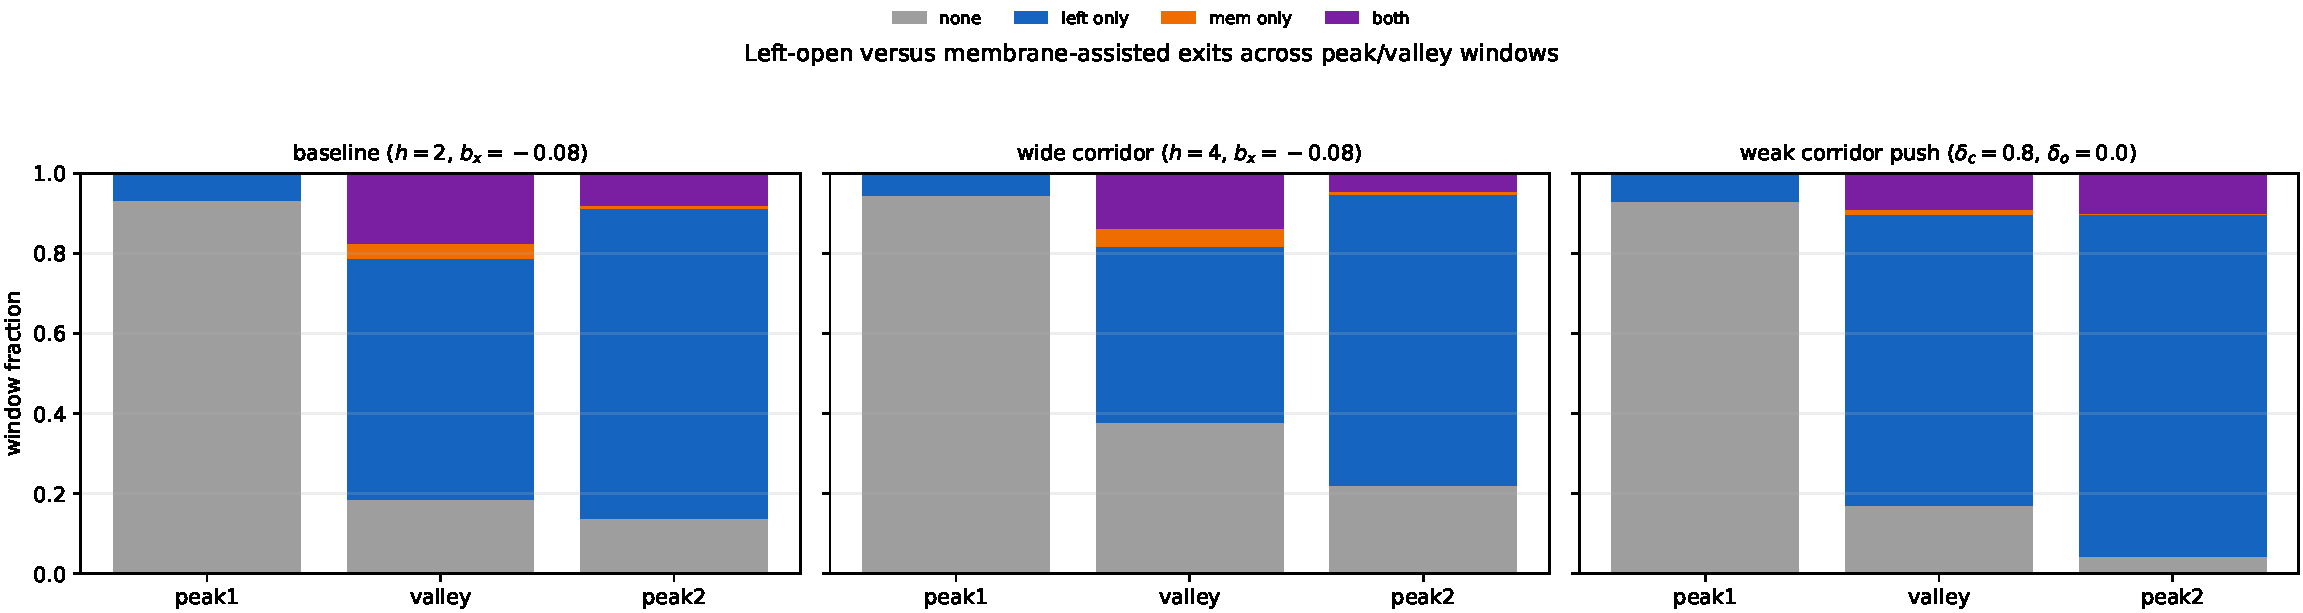
\includegraphics[width=0.95\linewidth]{../artifacts/figures/one_target_left_open_vs_membrane_windows.pdf}
  \caption{one-target 三个代表 sensitivity cases 的窗口分解。第一峰几乎完全由 \texttt{none} 支撑；到了 valley / peak2，质量主要转移到 \texttt{left\_only}，而 \texttt{mem\_only} 始终很小。}
\end{figure}

\begin{table}[!htbp]
  \centering
  \caption{left-open vs membrane summary。表中汇报 selected sensitivity cases 的 peak2 组成，以及 late window 中 ``先经左端开口离开 corridor'' 和 ``先发生膜 crossing'' 的条件概率。}
  \begin{tabular}{lrrrrrrrr}
\toprule
case & phase & sep & $t_{p2}$ & left & mem & both & $\Pr(\tau_l)$ & $\Pr(\tau_m)$ \\
\midrule
baseline & 2 & 1.633 & 1686 & 77.5\% & 0.6\% & 8.1\% & 85.6\% & 8.8\% \\
wide corridor & 2 & 2.015 & 1666 & 72.6\% & 0.7\% & 4.5\% & 77.1\% & 5.2\% \\
narrow weak-drag & 1 & 0.730 & 2149 & 64.8\% & 1.2\% & 28.2\% & 93.0\% & 29.4\% \\
strong corridor push & 2 & 1.920 & 1638 & 73.6\% & 0.9\% & 8.1\% & 81.6\% & 8.9\% \\
weak corridor push & 1 & 0.675 & 2327 & 85.4\% & 0.2\% & 10.1\% & 95.6\% & 10.4\% \\
\bottomrule
\end{tabular}

\end{table}

\paragraph{baseline 现在能说得更具体。}
在 shared symmetric baseline 下，\texttt{peak1} 窗口里
\texttt{none}=93.2\%、
\texttt{left\_only}=6.6\%、
\texttt{mem\_only}=0.18\%、
\texttt{both}=0.06\%；
而到了 \texttt{peak2}，组成变成
\texttt{left\_only}=77.5\%、
\texttt{mem\_only}=0.6\%、
\texttt{both}=8.1\%、
\texttt{none}=13.7\%。
这说明第一峰确实就是 corridor 内的 fast branch；第二峰则不是纯穿膜峰，而是主要由左端开口 detour 之后再回返/再推进的 delayed branch 组成。

\paragraph{扫描后的稳定口径是什么。}
把新增 sensitivity 扫描里所有 \texttt{phase=2} 的 case 合在一起，\texttt{peak2} 的平均组成大约是
\texttt{left\_only}=75.2\%、
\texttt{mem\_only}=0.7\%、
\texttt{both}=7.2\%、
\texttt{none}=17.0\%；
同时
\[
\Pr(\tau_{\rm left}<\tau_{\rm hit}\mid \texttt{peak2})\approx 82.3\%,\qquad
\Pr(\tau_{\rm mem}<\tau_{\rm hit}\mid \texttt{peak2})\approx 7.9\%.
\]
因此更准确的 one-target 结论应该是：半透膜确实会修饰 slow branch 的 timing 与纯度，但第二峰的主体质量主要来自左端开口 detour/rollback，而不是纯 membrane-only crossing。

\section{two-target：保持 gate-lifted family 线不动}
two-target 这条线的数值与共享代码没有被这次 one-target 重构改动；保留的主结论仍然是：晚峰主导 coarse family 稳定是 \texttt{F\_no\_return}，不是 \texttt{F\_rollback}。因此 two-target 这一节只保留 canonical figures、scan slices 和 verification，不再重复改写主机制。

\begin{table}[!htbp]
  \centering
  \caption{two-target representative cases。}
  \begin{tabular}{lrrrrrrr}
\toprule
case & phase & $P_{near}$ & $P_{far}$ & $t_{p1}$ & $t_v$ & $t_{p2}$ & sep$_{gate}$ \\
\midrule
anchor & 2 & 0.324 & 0.676 & 7 & 196 & 469 & 2.493 \\
clear\_instance & 2 & 0.350 & 0.650 & 13 & 207 & 471 & 2.380 \\
near\_mass\_loss & 2 & 0.089 & 0.911 & 27 & 193 & 470 & 2.229 \\
\bottomrule
\end{tabular}

\end{table}

\begin{table}[!htbp]
  \centering
  \caption{two-target validation。}
  \begin{tabular}{lrrrrr}
\toprule
case & $q_{far}(start)$ & $P_{far}$ & gap & closure & MC err \\
\midrule
anchor & 0.676009 & 0.676009 & 0.000000 & 0.000000 & 0.006816 \\
clear\_instance & 0.650264 & 0.650264 & 0.000000 & 0.000000 & 0.004222 \\
near\_mass\_loss & 0.911262 & 0.911262 & 0.000000 & 0.000000 & 0.005743 \\
\bottomrule
\end{tabular}

\end{table}

\begin{table}[!htbp]
  \centering
  \caption{63 点 $(d,\Delta y)$ atlas 的 phase 计数。}
  \begin{tabular}{rr}
\toprule
phase & count \\
\midrule
0 & 2 \\
2 & 61 \\
\bottomrule
\end{tabular}

\end{table}

\begin{figure}[!htbp]
  \centering
  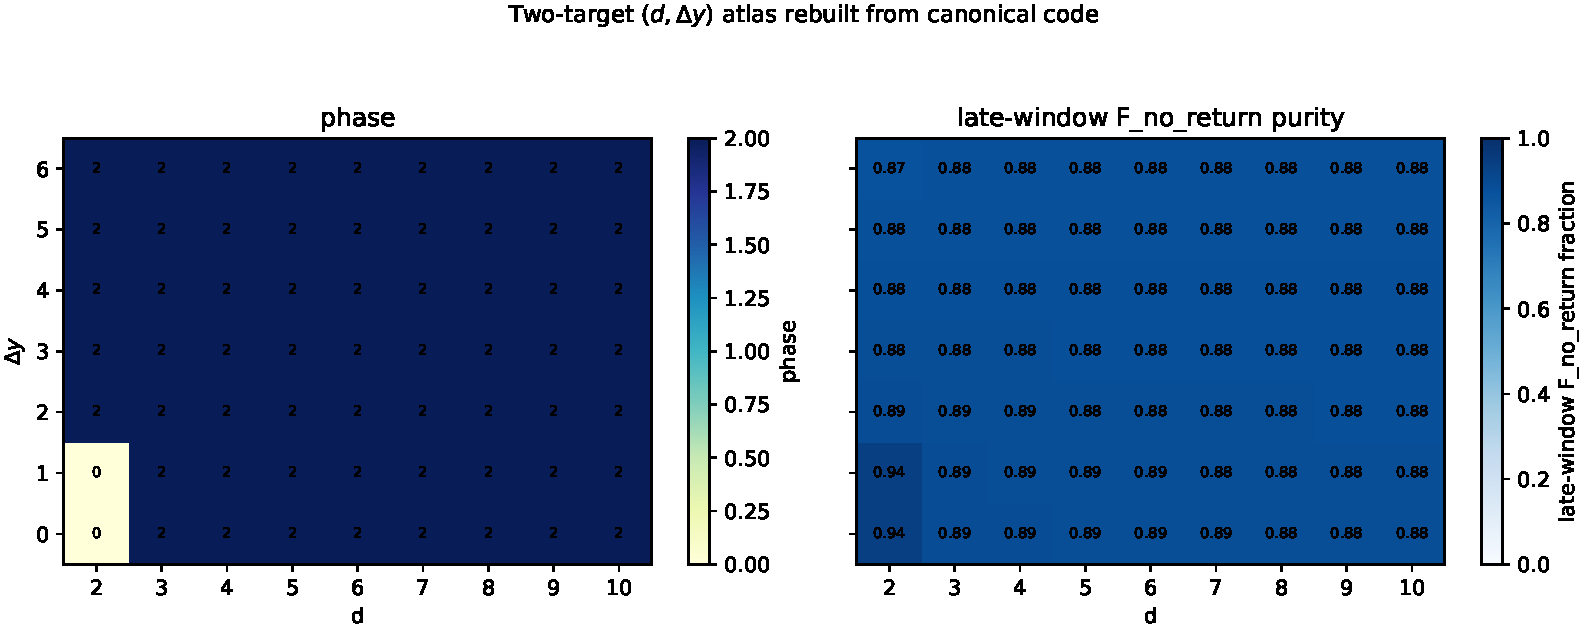
\includegraphics[width=0.88\linewidth]{../artifacts/figures/two_target_dx_dy_phase_purity.pdf}
  \caption{two-target 的 63 点 atlas。当前 canonical 重算结果仍然保持 phase-0 仅在少数点出现。}
\end{figure}

\begin{figure}[!htbp]
  \centering
  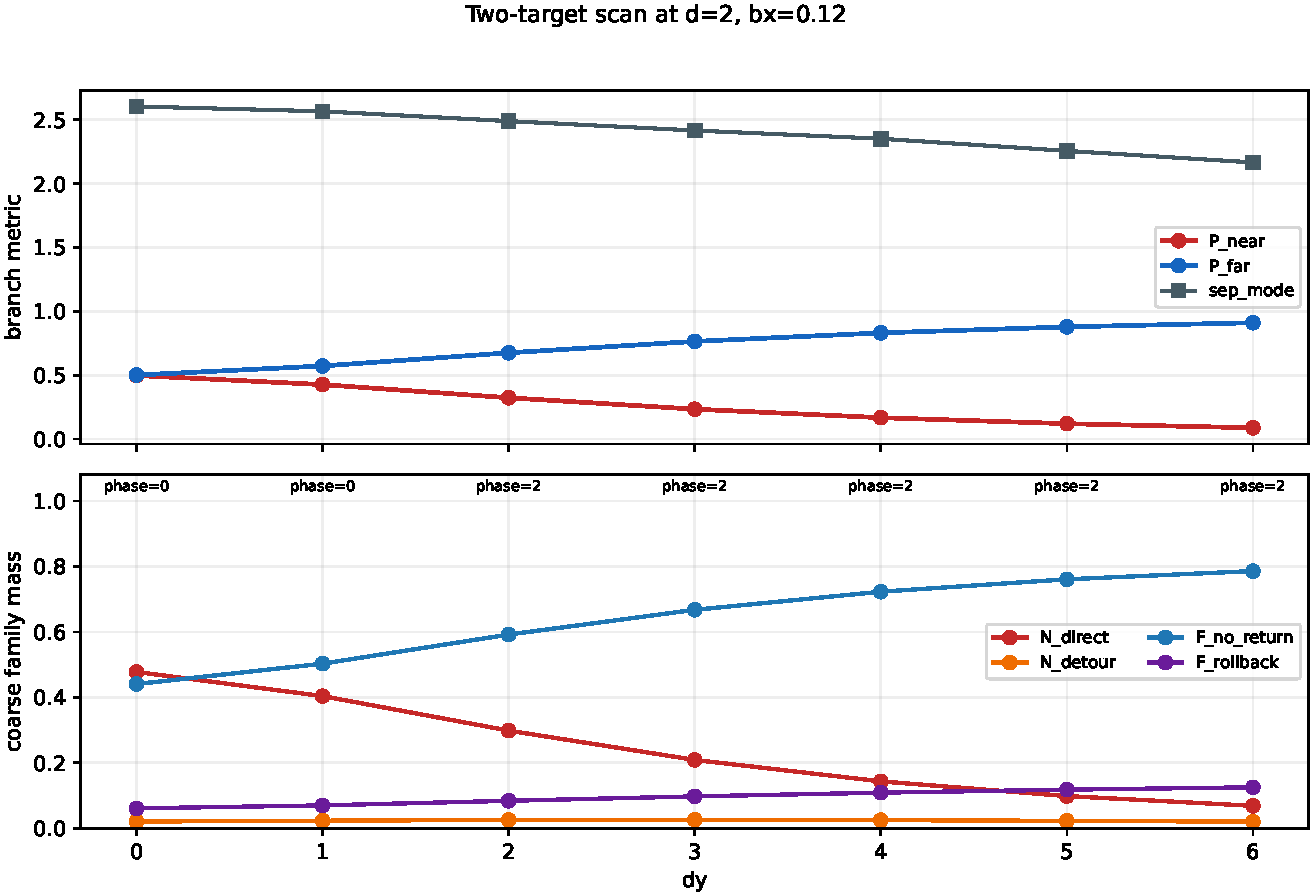
\includegraphics[width=0.88\linewidth]{../artifacts/figures/two_target_scan_dy_d2_bx0p12.pdf}
  \caption{固定 $d=2$ 的 $\Delta y$ 扫描。}
\end{figure}

\begin{figure}[!htbp]
  \centering
  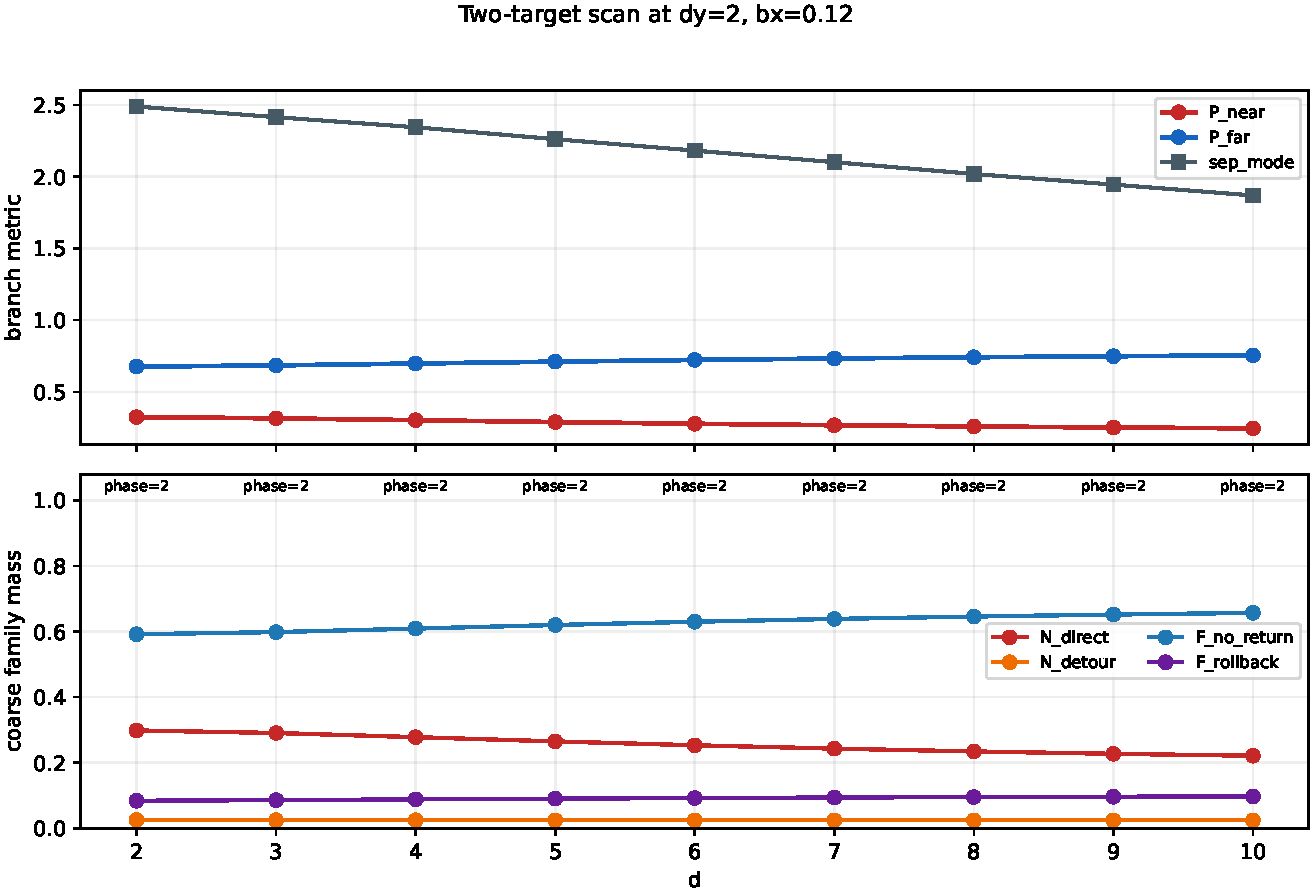
\includegraphics[width=0.88\linewidth]{../artifacts/figures/two_target_scan_d_dy2_bx0p12.pdf}
  \caption{固定 $\Delta y=2$ 的 $d$ 扫描。}
\end{figure}

\begin{figure}[!htbp]
  \centering
  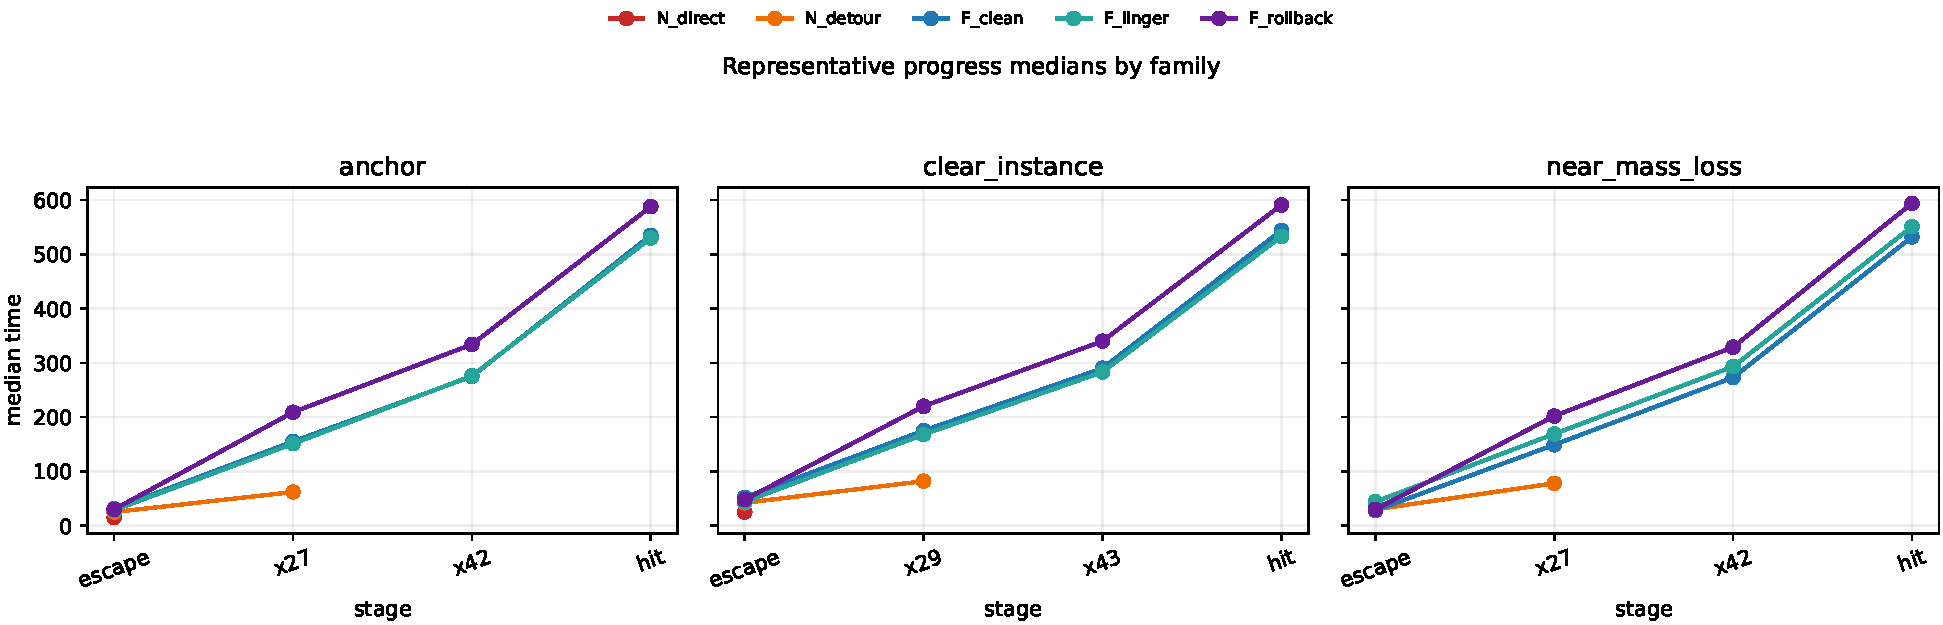
\includegraphics[width=0.86\linewidth]{../artifacts/figures/two_target_progress_medians.pdf}
  \caption{representative progress medians。}
\end{figure}

\begin{figure}[!htbp]
  \centering
  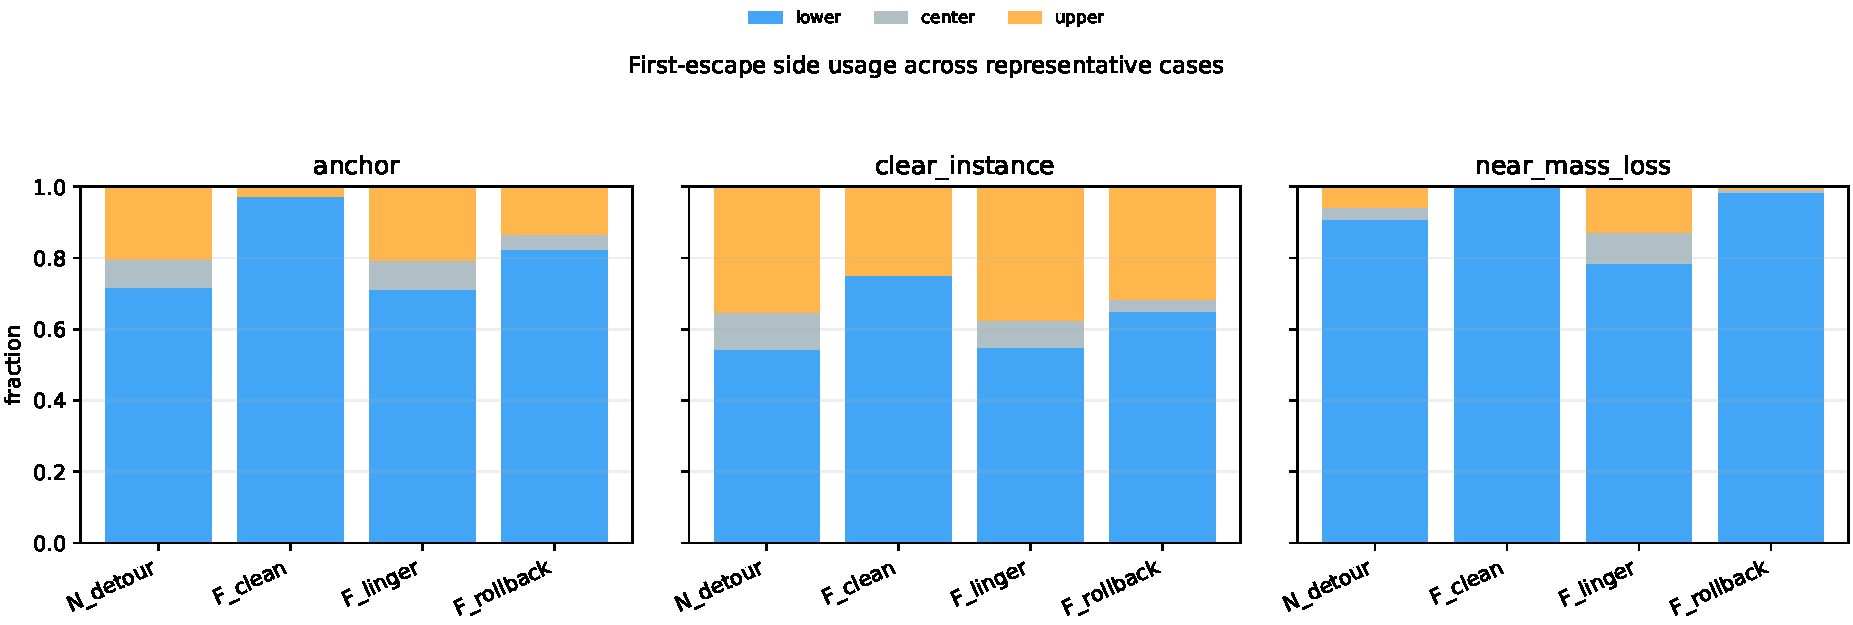
\includegraphics[width=0.86\linewidth]{../artifacts/figures/two_target_first_escape_side_usage.pdf}
  \caption{representative first-escape side usage。}
\end{figure}

\begin{figure}[!htbp]
  \centering
  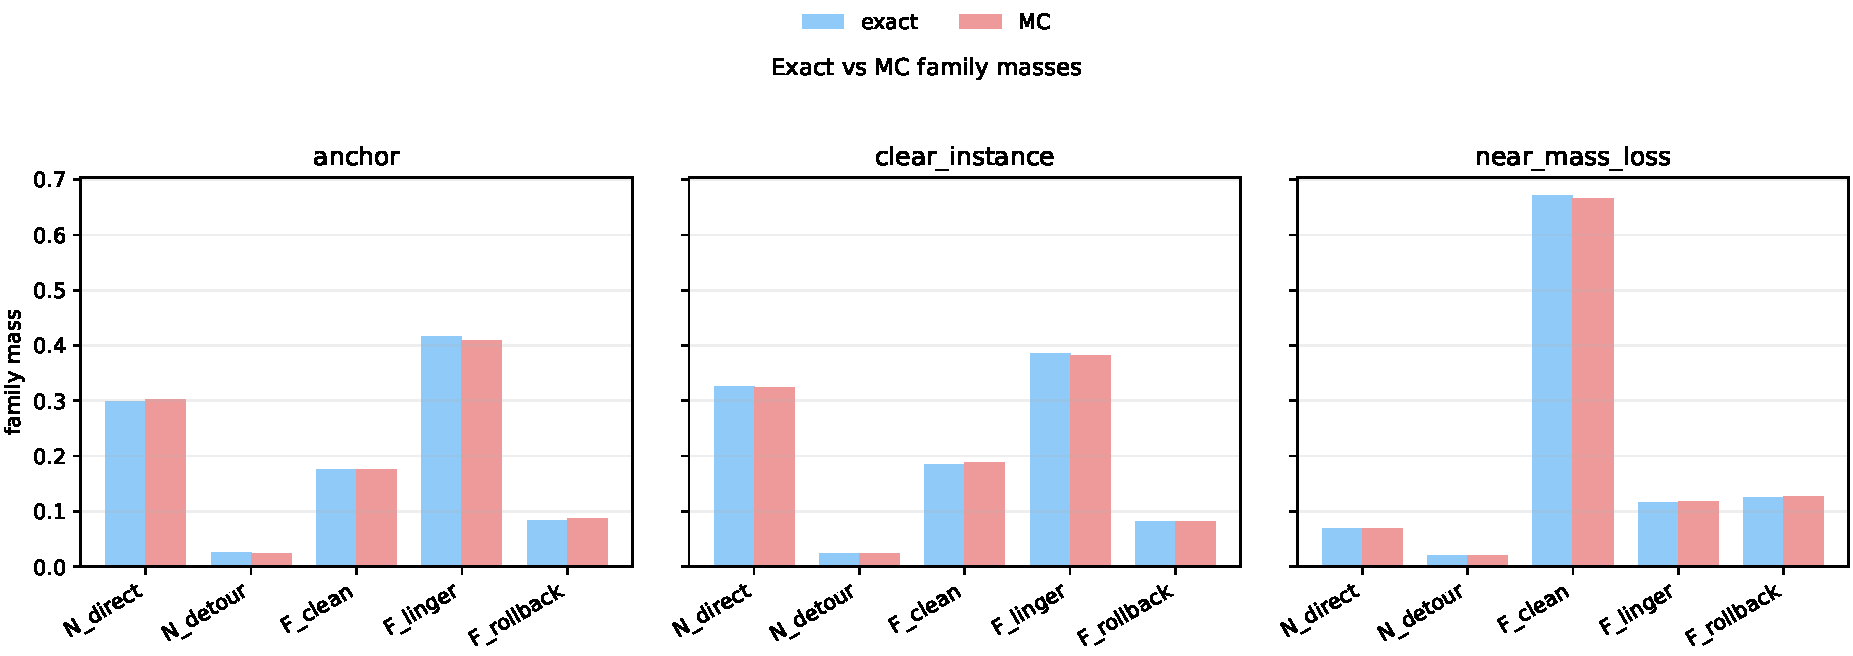
\includegraphics[width=0.86\linewidth]{../artifacts/figures/two_target_mc_vs_exact.pdf}
  \caption{MC-vs-exact 对照。}
\end{figure}

\begin{figure}[!htbp]
  \centering
  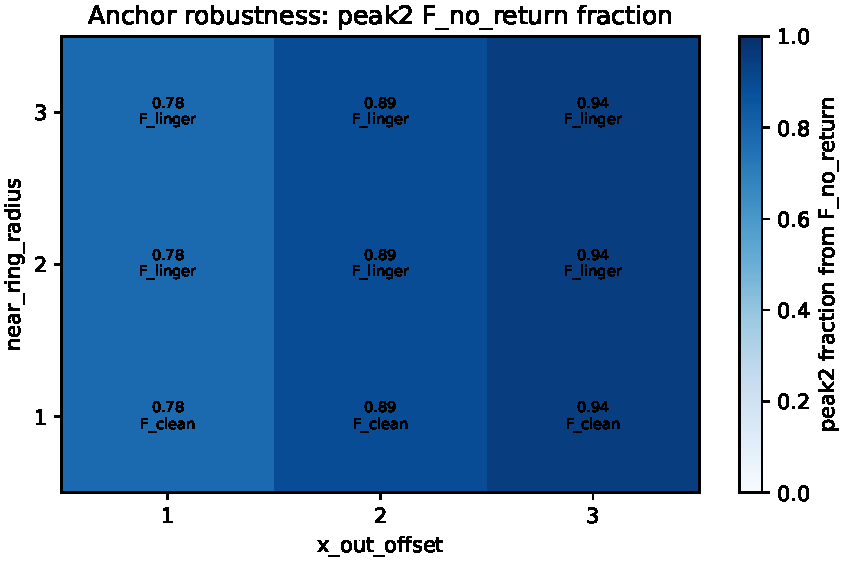
\includegraphics[width=0.86\linewidth]{../artifacts/figures/two_target_anchor_gate_robustness.pdf}
  \caption{anchor case 的 gate robustness。}
\end{figure}

\begin{table}[!htbp]
  \centering
  \caption{two-target representative recheck。}
  \begin{tabular}{lrrrrr}
\toprule
case & source $P_{far}$ & recheck $P_{far}$ & $q_{far}(start)$ gap & late family & MC err \\
\midrule
anchor & 0.676009 & 0.676009 & 0.000000 & F\_no\_return & 0.0068 \\
clear\_instance & 0.650264 & 0.650264 & 0.000000 & F\_no\_return & 0.0042 \\
near\_mass\_loss & 0.911262 & 0.911262 & 0.000000 & F\_no\_return & 0.0057 \\
\bottomrule
\end{tabular}

\end{table}

\section{仓库接入与附录说明}
\paragraph{仓库接入。}
当前 canonical 报告继续把 6 个原始下载文件完整归档在
\texttt{notes/source\_imports/2026-03-16/raw/}
下；新的 \texttt{artifacts/} 和 \texttt{manuscript/} 则全部由共享模块
\texttt{vkcore.grid2d.one\_two\_target\_gating.*}
重建。

\paragraph{one-target 当前的最终口径。}
如果用一句话概括这一稿 one-target 的最终口径，就是：
\begin{quote}
标准配置是共享对称基线；第一峰是 corridor fast branch；第二峰主要是左端开口 detour/rollback branch；半透膜 crossing 是 slow branch 的次级修饰；x-gate 只负责膜 first-leak timing；双峰丢失只按 \texttt{phase=0} 计算；极端 $\kappa=0$ 只做 control。
\end{quote}

\section{附录：committor control}
committor 仍然保留在仓库里，但只作为附录 control。它仍然适合做历史连续性与数值对照，却不再定义 one-target 主文中的 gate。

\begin{figure}[!htbp]
  \centering
  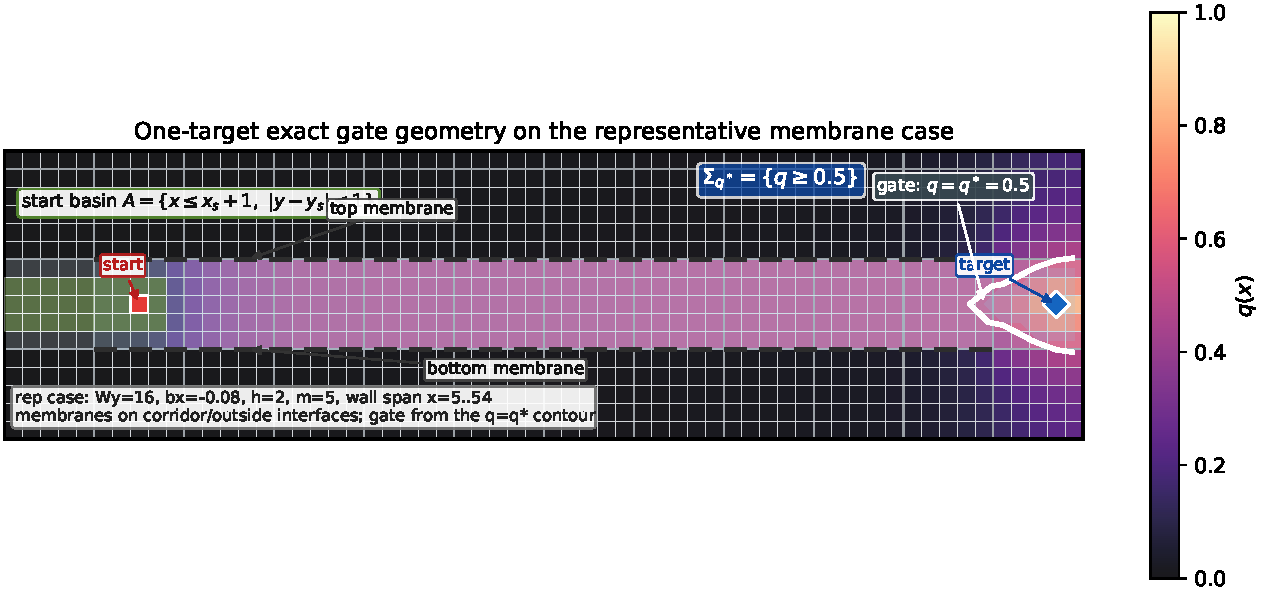
\includegraphics[width=0.86\linewidth]{../artifacts/figures/one_target_committor_control_geometry.pdf}
  \caption{one-target 的 committor 对照图。这里的 $q=q^*$ 轮廓线仍然存在，但它已经退出主叙事。}
\end{figure}

\end{document}
